\chapter{跨域自适应多目标检测与跟踪算法研究}
多目标跟踪系统在真实开放场景(如智能交通、自动驾驶)中的部署,常受雾、低光照等恶劣天气条件的制约。
这些条件导致成像质量退化,形成训练(清晰图像)与测试(恶劣天气图像)之间的输入域差异,
进而造成检测与跟踪性能的显著下降。
尽管第三章提出的跟踪器在清晰域数据上表现出色,
但其性能在跨域场景下仍受限于前端检测模块的退化。

为构建真正鲁棒的跟踪系统,必须在跟踪前端解决输入层面的域自适应问题。
本章针对此问题,提出一套完整的跨域自适应解决方案:
首先,通过可视化分析明确恶劣环境对检测与跟踪的影响(\ref{sec:ch4_1}节);
其次,提出一种基于双渐进滤波的跨域自适应增强器,并与检测器进行端到端协同训练,
实现输入图像的自适应增强(\ref{sec:ch4_2}节);
进而,将训练好的增强-检测模块与冻结的第三章跟踪器集成,
构建完整的“增强-检测-跟踪”推理框架(\ref{sec:ch4_3}节);
最后,通过系统的实验验证所提方法在检测与跟踪任务上的有效性(\ref{sec:ch4_4}节)。
本章工作旨在从源头缓解域偏移,为下游跟踪任务提供鲁棒的视觉表示,是实现跨域自适应跟踪的关键一环。

\section{跨域与恶劣环境问题分析}
\label{sec:ch4_1}
正如本章引言所强调,基于“检测-跟踪”范式的多目标跟踪系统在鲁棒性上表现出显著的强前端依赖性。
尽管后端关联算法(如本文第三章提出的DGCTracker)具备卓越的时空信息建模能力,但其性能上界在本质上仍受限于前端检测器的输出质量。
本节将从数据分布、检测响应、跟踪关联三个层面,逐层分析跨域恶劣环境下的系统退化机理。

\subsection{跨域场景下的数据分布偏移}
现有的主流目标检测器(如 YOLO 系列)大多在MS COCO\cite{coco}、ImageNet\cite{imagenet}等高质量数据集上进行训练,这些源域数据通常具有直方图均衡、纹理清晰、信噪比高的统计特征。
然而,恶劣天气条件下的目标域数据在像素级统计分布上发生了本质改变:

\begin{itemize}
    \item \textbf{雾天场景(Foggy Domain)}:受大气散射模型影响,图像呈现出非均匀的“白化”干扰。随景深增加,物体表面的对比度呈指数级衰减,高频纹理信息丢失,导致特征提取器难以捕捉清晰的边缘梯度。
    \item \textbf{弱光场景(Dark Domain)}:由于成像亮度不足,图像的有效动态范围被压缩至低灰度区间,并伴随明显的色彩失真现象。目标与背景之间的判别性降低,从而削弱了基于外观信息的特征表达能力。
\end{itemize}

上述变化导致目标域数据与源域数据在统计分布上不再满足独立同分布(Independent and Identically Distributed, I.I.D.)假设,使得在源域条件下学习到的卷积滤波器难以在目标域中保持原有的判别能力,从而导致检测与跟踪性能的级联退化。

\subsection{恶劣环境对目标检测性能的影响}
为直观分析恶劣环境对检测性能的影响,本节以 MOT17-02 场景为例,在保持检测模型参数不变的前提下,将原始序列及其弱光、加雾退化版本分别输入 YOLOv3 检测器进行推理,并对检测结果进行定性对比分析。
相关可视化结果如\autoref{fig:ch4_1}所示。
\begin{figure}[htbp]
    \centering
    \includegraphics[width=16cm]{chapter4/1.png}
    \caption{\label{fig:ch4_1}跨域场景下检测性能退化的可视化对比}
\end{figure}

从检测结果可以观察到,恶劣环境主要从以下三个方面削弱了目标检测器的输出质量:
\begin{itemize}
    \item \textbf{目标漏检率显著上升}:恶劣环境显著提高了目标的漏检率,尤其是对远距离及小尺度目标影响更为严重。在雾天场景中,大气散射效应削弱了目标的局部对比度,使得目标区域与背景难以区分;而在弱光场景中,成像噪声与亮度压缩共同作用,进一步降低了目标的可检测性。
    \item \textbf{检测置信度降低}:对于未被漏检的目标,其检测置信度虽仍能维持在较高水平,但与清晰场景下普遍高于0.9的置信度相比,存在明确且系统性的下降。这一现象表明,跨域条件下特征表示的稳定性受到影响,使得检测器对目标的分类置信度相对下降。
    \item \textbf{定位精度下降}:由于环境退化模糊了目标的边缘梯度,使得回归网络难以收敛到一致的边界。这种定位精度的丧失,不仅降低了单帧测量的可靠性,也增加了后续基于几何距离进行数据关联的模糊度。
\end{itemize}

综合上述分析可以看出,跨域与恶劣环境条件并非仅导致检测性能指标的数值下降,而是从置信度分布、目标召回以及定位稳定性等多个层面削弱了检测结果作为可靠观测的质量。
这种观测层面的退化将进一步影响依赖检测结果进行状态估计与数据关联的多目标跟踪过程。

\subsection{恶劣环境对多目标跟踪性能的影响}
多目标跟踪(MOT)本质上是一个基于最大后验概率(Maximum A Posteriori Estimation,MAP)的时序推理过程,其核心高度依赖于观测数据的完备性与准确性。
当前端检测器在恶劣环境下输出稀疏(漏检)且含噪(定位漂移)的检测集合时,后端跟踪器的数据关联与轨迹管理等核心机制将发生系统性的失效。如\autoref{fig:ch4_2}所示,这种失效主要表现为两种典型情况:
\begin{figure}[htbp]
    \centering
    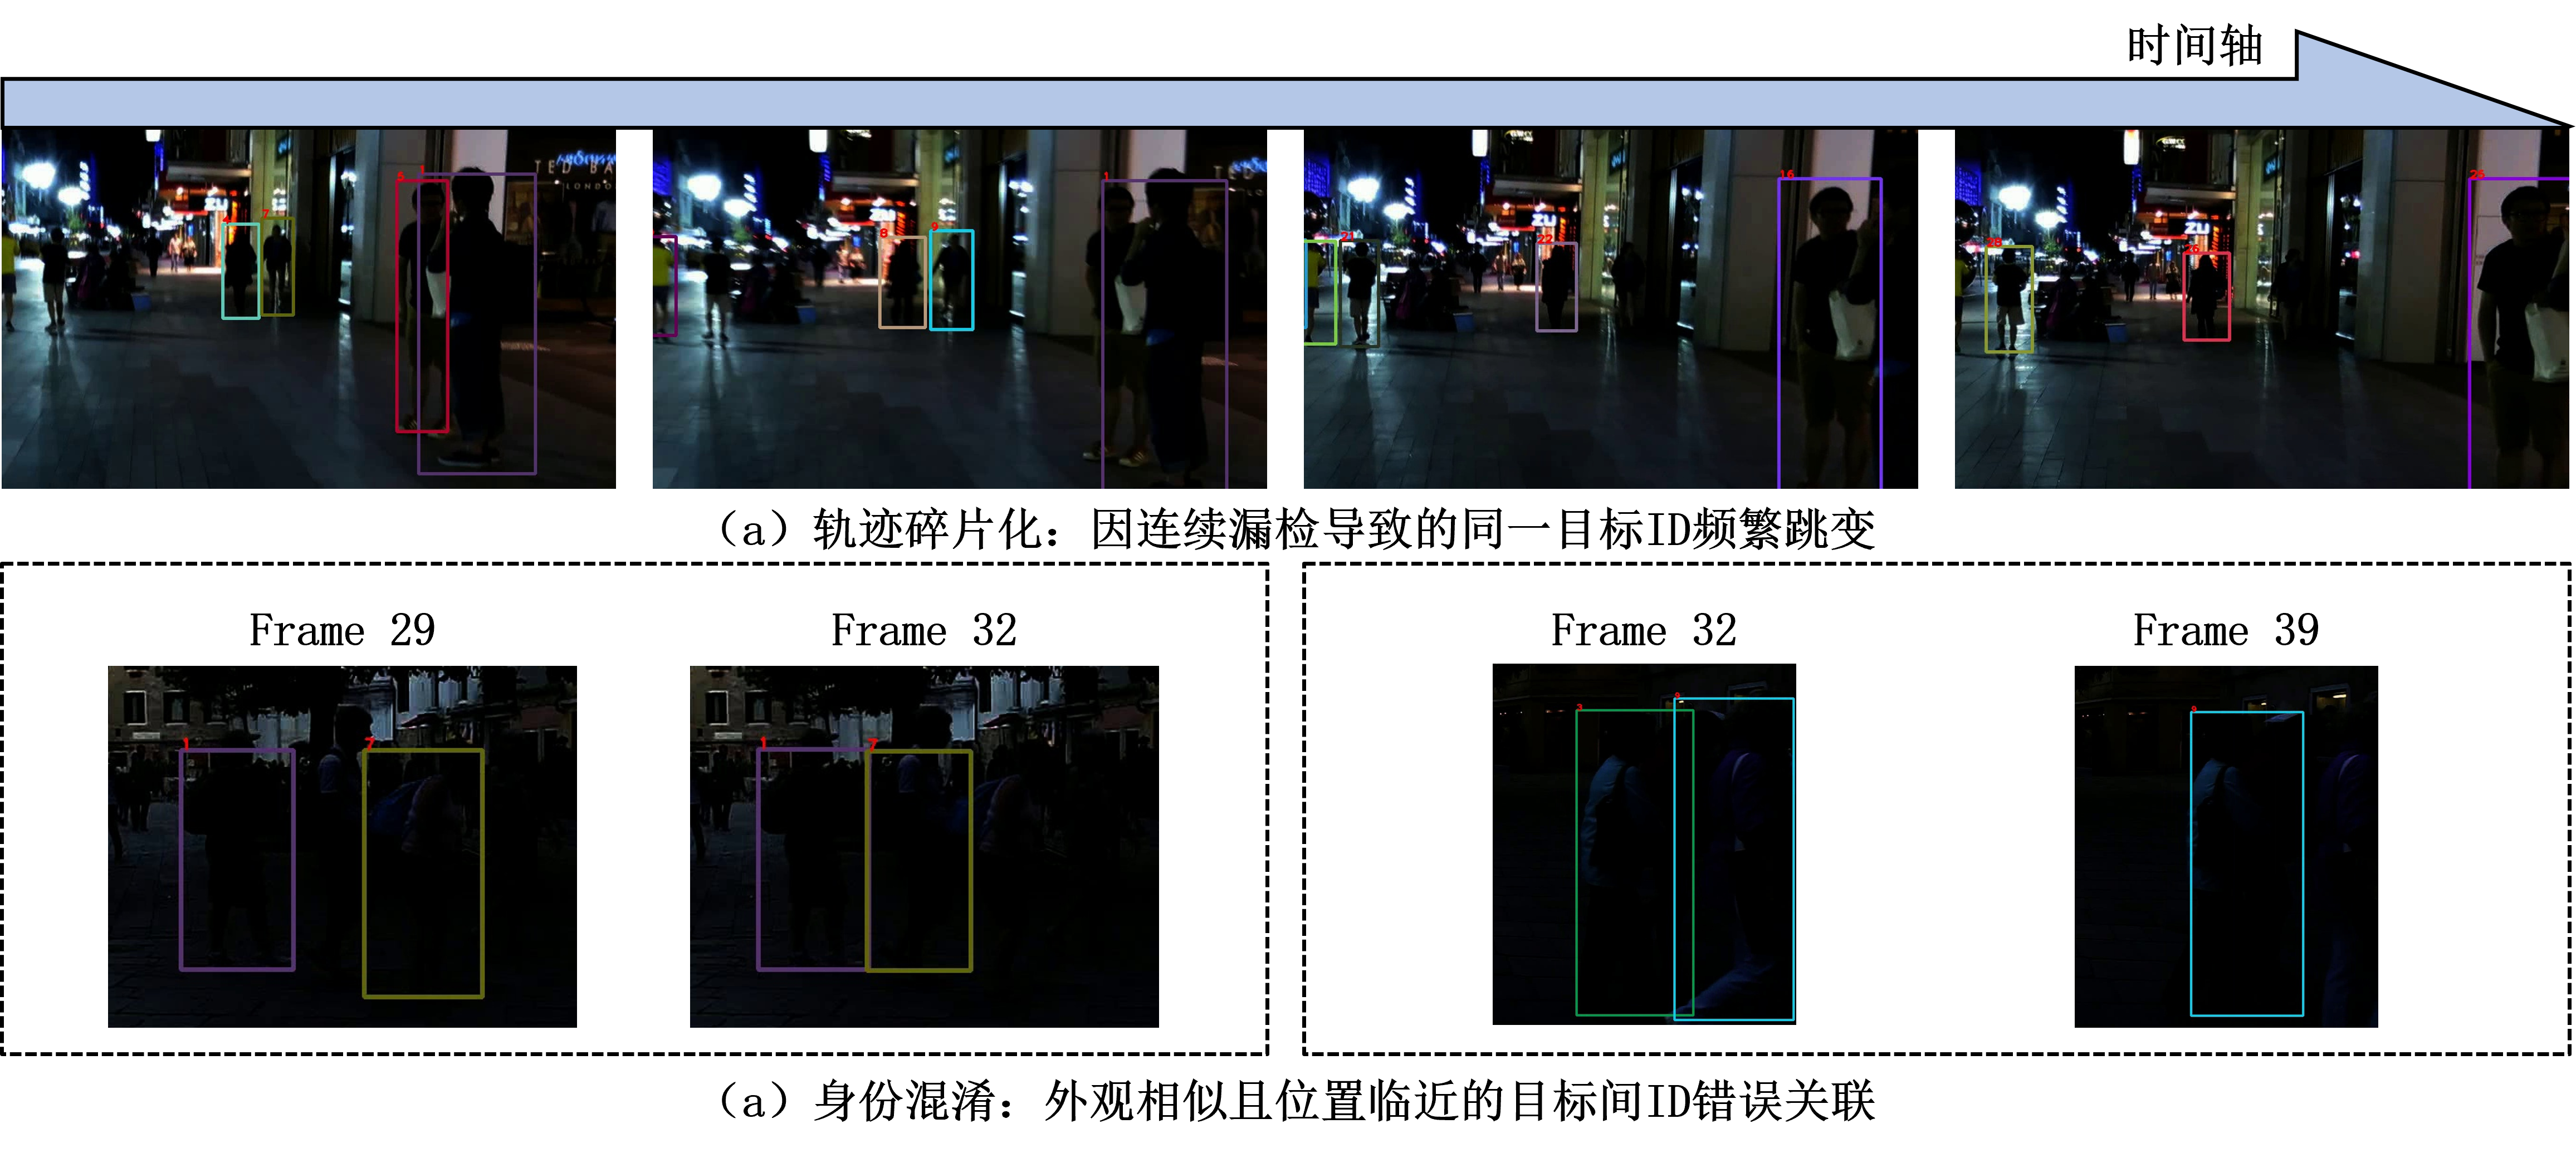
\includegraphics[width=16cm]{chapter4/2.png}
    \caption{\label{fig:ch4_2}弱光环境下多目标跟踪性能退化典型案例}
\end{figure}

\begin{itemize}
    \item \textbf{轨迹碎片化(Trajectory Fragmentation)}:如\autoref{fig:ch4_2}(a)所示,在持续跟踪同一行人的过程中,由于高频的间断性漏检,该目标的检测序列在时间轴上不再连续。这导致跟踪器无法将其关联为一条完整轨迹,而是将其错误地初始化为四条独立的短轨迹(ID=4, 8, 22, 26),造成严重的轨迹碎片化。这种现象使得目标的时序连续性被破坏,大幅增加了轨迹管理的复杂度。
    \item \textbf{身份混淆(Identity Confusion)}:如\autoref{fig:ch4_2}(b)所示,在弱光环境下,空间位置相近且外观相似的多个目标容易发生身份分配错误。该现象主要与恶劣环境下外观特征判别性下降有关。由于成像退化削弱了颜色、纹理等外观线索,由检测框中提取的表观特征在特征空间中的可分性显著降低,使得基于相似度的关联决策变得不稳定,从而增加了身份混淆与错误关联的发生概率。
\end{itemize}

上述两类现象在时间维度上的不断累积,最终表现为多目标跟踪结果整体一致性的显著下降。
轨迹碎片化破坏了目标运动轨迹的完整性,而身份混淆则直接削弱了身份保持能力。
这表明,在跨域与恶劣环境条件下,若不从输入层面改善检测质量与外观表征,仅依赖后端关联算法难以从根本上缓解多目标跟踪性能的退化问题。
因此,本章后续工作将聚焦于设计一个可学习、可集成的前端图像增强模块,旨在直接从输入图像层面补偿域偏移,恢复可靠的观测质量,从而为下游检测与跟踪任务提供保障。
\section{跨域自适应前端增强检测框架}
\label{sec:ch4_2}
针对\ref{sec:ch4_1}节所揭示的恶劣环境下检测性能退化的问题,本节提出一种前端自适应方案——双渐进滤波增强器(Dual Progressive Filter Enhancer,DPFE),并将其与目标检测器(YOLOv3)进行端到端协同训练,构建
一个统一的跨域自适应增强与检测系统(DPFE-YOLO)。该系统旨在通过可学习的图像增强器,将恶劣天气下的退化图像映射到清晰域,从而恢复检测器所需的高质量视觉特征,从输入层缓解域偏移。
\begin{figure}[htbp]
    \centering
    \includegraphics[width=13cm]{chapter4/3.png}
    \caption{\label{fig:ch4_3}DPFE-YOLO整体框架概览}
\end{figure}

整体框架结构如\autoref{fig:ch4_3}所示,主要由两个核心子系统串联而成:前端的双渐进滤波增强器(DPFE)与后端的目标检测器(如YOLOv3)。
具体而言,原始退化图像首先输入双渐进滤波增强器中。在该模块中,图像先经过视觉编码器提取多层次特征,这些特征随后用于引导一系列级联的双流滤波块(Dual Filter Block,DFB)进行渐进式的恢复处理。

为了兼顾全局光照调整与局部去噪的需求,每个DFB内部均采用双路并行的处理架构,包含两个核心可微滤波器与一个门控融合模块:
\begin{itemize}
    \item \textbf{贝塞尔像素级滤波器(Bezier Pixel-wise Filter,BPW)}:该分支利用贝塞尔曲线进行全局像素映射,主要负责图像的亮度增强与对比度拉伸;
    \item \textbf{基于核的局部滤波器(Kernel-based Local Filter,KBL)}:该分支通过动态预测卷积核进行空间滤波,专注于去除雾霾纹理并恢复边缘细节。
\end{itemize}
上述两路滤波分支的输出通过门控机制(Gate)进行自适应加权融合。该机制根据输入特征动态生成权重,决定像素级增强与局部滤波在最终结果中的贡献占比。

最后,经过多级DFB逐步增强后的图像被直接送入YOLOv3检测器中,完成目标定位与分类任务。整个系统通过增强损失与检测损失进行端到端联合训练,确保
前端增强器生成的图像特征能最大化地服务于后端的检测性能。

为系统阐述该方法,本节首先介绍所采用的基础可微滤波组件(\ref{subsec:ch4_2_1}节);随后详细阐述
双渐进滤波增强器的结构设计与工作原理(\ref{subsec:ch4_2_2}节);接着说明增强器与检测器协同训练策略(\ref{subsec:ch4_2_3}节);
最后,可视化增强器的内部状态,展示DPFE的渐进增强与自适应修复机制(\ref{subsec:ch4_2_4}节)。
\subsection{基础滤波组件}
\label{subsec:ch4_2_1}
在双渐进滤波增强器中,图像增强的核心依赖于两个基础滤波组件:贝塞尔像素级滤波器(BPW)和基于核的局部滤波器(KBL)。这两个滤波器均继承自ERUP-YOLO\cite{erup}工作,
分别负责全局像素强度映射与局部空间滤波,共同构成了后续双流滤波块(DFB)的核心处理单元。

这种设计是对\ref{subsec:ch2_2_3}节所述的经典可微图像处理方法的进一步升华。现有的 DIP 方法(如 IA-YOLO \cite{ia})通常直接借用传统 ISP 中的固定数学模型(如伽马校正的幂函数、锐化滤波器的线性组合等)。
虽然这些方法具备物理可解释性,但其参数空间往往是不连续的,且单一的物理模型难以拟合复杂多变的恶劣天气退化分布。相比之下,BPW和KBL提供了更具通用性的参数化表达:
BPW是对各类单调色调映射曲线的全局拟合,而KBL则是对各类空间滤波操作的局部统一。本节将详细阐述这两个组件的数学原理和参数化形式。

\textbf{1. 贝塞尔像素级滤波器(BPW)}

BPW滤波器的目标是为图像的每个通道(RGB)学习一个单调递增的非线性映射函数,从而统一实现传统图像处理中的伽马矫正、对比度拉伸和色调映射等全局操作。
该映射通过一个参数化的三次贝塞尔曲线实现。

如\autoref{fig:ch4_4}所示,一条三次贝塞尔曲线由四个控制点定义:起点$P_0=(0,0)$,终点$P_3=(1,1)$,以及两个可学习的控制点$P_1$和$P_2$。
曲线上的点$C(t)=(C_x(t),C_y(t))$由参数$t\in [ 0,1 ]$表示为:
\begin{equation}
    C(t) = (1-t)^3P_0 + 3(1-t)^2tP_1+3(1-t)t^2P_2+t^3P_3
\end{equation}

为保证映射的单调性及输出范围在$[0,1]$,ERUP-YOLO将控制点$P_1$和$P_2$约束在单位正方形内。
具体地,控制点坐标由可学习参数$r_1$,$\theta_1$,$r_2$,$\theta_2$(每个通道独立)通过下式计算:
\begin{equation}
    \begin{aligned}
        P_1 &= \left(\frac{r_1+1}{2} \cos( \frac{(\theta_1+1)\pi}{4}), \frac{r_1+1}{2}\sin(\frac{(\theta_1+1)\pi}{4})\right) \\
        P_2 &= \left(\frac{r_2+1}{2} \cos( \frac{(\theta_2+1)\pi}{4}), \frac{r_2+1}{2}\sin(\frac{(\theta_2+1)\pi}{4})\right)
    \end{aligned}
\end{equation}
其中,$r_1,r_2\in[-1,1]$,$\theta_1,\theta_2\in[-1,1]$。当所有参数为零时,曲线退化为恒等映射$y=x$。
\begin{figure}[htbp]
    \centering
    \includegraphics[width=13cm]{chapter4/4.png}
    \caption{\label{fig:ch4_4}贝塞尔曲线像素级滤波器(BPW)的映射曲线示例}
\end{figure}

为实现高效的可微运算,ERUP-YOLO采用分段线性近似:将参数区间$t\in[0,1]$均匀划分为$L$段(通常$L=8$),在第$j$段($t\in[t_j,t_{j+1}]$)内,使用线性函数近似曲线,
其斜率为$\Delta C_y(t_j)/\Delta C_x(t_j)$。则对于输入像素强度$p_{in}\in [0,1]$,输出强度$p_{out}$通过下式计算:
\begin{equation}
p_{out} = \sum_{j=0}^{L-1}\text{clip}\left(p_{in} - C_x(t_j),0,\Delta C_x(t_j)\right)\cdot \frac{\Delta C_y(t_j)}{\Delta C_x(t_j)}
\label{equ:bpw}
\end{equation}
其中,$\text{clip}(x,a,b)$将$x$裁剪到区间$[a,b]$,$\Delta C_x(t_j) = C_x(t_{j+1} - C_x(t_j))$,$\Delta C_y(t_j) = C_y(t_{j+1} - C_y(t_j))$。
该操作对每个RGB通道独立进行,因此BPW滤波器共有$3\times 4=12$个可学习的参数(每通道四个)。

如\autoref{fig:ch4_5}所示,BPW滤波器通过一条可学习的曲线统一个多种全局变换。当曲线呈现上凸形态时,其作用类似于伽马校正($\gamma < 1$)以增强暗部细节;
当下凹时则类似于对比度拉伸;而通过为不同通道学习不同的曲线形状,即可实现自适应白平衡与色调调整。因此,BPW可以视为对\ref{subsec:ch2_2_3}中多个独立像素级滤波器的泛化与统一。
\begin{figure}[htbp]
    \centering
    \includegraphics[width=16cm]{chapter4/5.png}
    \caption{\label{fig:ch4_5}贝塞尔曲线像素级滤波器(BPW)与传统像素级滤波器的映射曲线对比(摘自ERUP-YOLO)}
\end{figure}

\textbf{2. 基于核的局部滤波器(KBL)}

KBL滤波器旨在模拟去雾、锐化等依赖于局部邻域的空间滤波操作。其设计灵感来源于传统ISP中的锐化滤波器与基于物理的去雾模型,但将其统一为一种可学习的局部线性卷积形式。

KBL滤波器对输入图像$I$(各通道独立处理)执行如下处理:
\begin{equation}
    F_{KBL}(I) = I \otimes K_1 + I \otimes K_2 + I
\end{equation}
其中$\otimes$表示卷积操作,$K_1$和$K_2$为两个可学习的卷积核(尺寸为$k\times k$,默认设置为$k=9$),分别对应局部调制与细节恢复两项。第一项$I\otimes K_1$可视为对输入图像的局部加权平均,
起到自适应平滑或锐化作用;第二项$I\otimes K_2$则用于添加恢复性的细节成分;最后一项残差连接保留了原始输入信息,确保梯度顺畅传播。

在ERUP-YOLO中,卷积核$K_1$和$K_2$的参数是由一个小型神经网络从输入图像的特征中动态预测,并通过$\text{tanh}$函数将数值约束在$[-1,1]$区间。然而,这种简单的约束方式
并不能保证卷积核的稳定性,尤其是在训练初期,预测的卷积核可能具有较大的幅值,导致梯度爆炸或训练不稳定。为了增强训练的稳定性和卷积核的可解释性,我们在其基础上提出了一种改进的归一化策略。

具体而言,对于每个通道$c$,预测的核参数首先通过$\text{tanh}$函数约束在$[-1,1]$区间,得到原始卷积核$\tilde{K}_1^c,\tilde{K}_2^c \in \mathbb{R}^{k\times k}$。
然后我们对每个卷积核进行如下归一化操作:
\begin{equation}
    K_i^c = \frac{\tilde{K}_i^c}{ \sum_{u,v}\tilde{K}_1^c(u,v) + \epsilon}, \quad i = 1,2
\end{equation}
其中$\epsilon$为一个小常数(默认设置为$10^{-8}$),用于防止除零。归一化后的卷积核满足$\sum_{u,v}\tilde{K}_1^c(u,v) \approx 1 $,从而将卷积操作的输出幅值限制在合理范围内。

这种改进的归一化策略具有以下优点:
\begin{enumerate}
    \item \textbf{训练稳定性}:通过约束卷积核的$L1$范数,有效避免了因核权值幅值过大而导致的梯度爆炸或数值溢出,使训练过程更加平稳。
    \item \textbf{可解释性}:归一化后的卷积核可以视为对输入局部区域的加权平均,其权重绝对值之和为1,符合传统空间滤波器的物理含义,便于理解与分析。
    \item \textbf{泛化能力}:归一化操作使滤波器在不同图像和不同退化条件下具有一致的数值尺度,有助于提升模型的泛化性能。
\end{enumerate}

KBL滤波器通过对每个通道使用独立的归一化卷积核,能够灵活地处理不同颜色通道上的退化模式。该滤波器总计有$2\times 3 \times k^2$个可学习参数(两个核、三个通道、每个核$k^2$个参数),
在保持强大表达能力的同时,通过归一化确保了数值稳定性。

KBL滤波器将\ref{subsec:ch2_2_3}节中提到的多种局部滤波操作抽象为一种通用的、数据驱动的局部卷积形式。
其双核设计使得网络能够同时学习平滑噪声与增强细节两种互补操作,从而更灵活地应对雾霾、噪声等多种局部退化。

综上所述,BPW与KBL滤波器分别提供了全局非线性映射与局部空间滤波两种可微的图像处理基元。
它们将传统图像处理操作参数化并嵌入到深度学习框架中,
为后续构建自适应、可学习的增强模块奠定了坚实基础。
与第二章介绍的经典可微滤波器相比,BPW与KBL通过更统一的数学形式和更少的先验假设,
实现了对图像退化更强大的建模能力,是构建下一步图像自适应前端的关键组件。
\subsection{双渐进滤波增强器结构设计}
\label{subsec:ch4_2_2}
基于\ref{subsec:ch4_2_1}节介绍的基础可微滤波组件,本节详细阐述双渐进滤波增强器(DPFE)的整体架构与内部工作机制。
如图\ref{fig:ch4_3}所示,DPFE由视觉编码器(Vision Encoder)与级联的双流滤波块(DFB)构成,
其设计遵循“强度渐进、层次引导”的增强原则,旨在通过多层次的特征引导与自适应滤波,将退化图像逐步恢复至清晰域。以下将依次介绍各核心组件的设计及其协同工作流程。

\textbf{1. 视觉编码器(Vision Encoder)}

视觉编码器作为DPFE的感知前端,负责从输入退化图像中提取多层次特征,
并将每个尺度的特征压缩为固定维度的条件向量,作为对应层次的双流滤波块(DFB)条件输入。
我们的视觉编码器设计在ERUP-YOLO的基础上进行了改进,使其特征提取过程更为平滑,以更好地保留空间信息。

如\autoref{fig:ch4_6}所示,现有的增强方法(如ERUP-YOLO、GDIP-YOLO等)通常采用传统的类似VGG\cite{vgg}的直筒结构:使用固定的平均池化(Average Pooling)进行下采样,并在末端通过高维度的全连接层
将特征压缩为参数。这种设计存在三个显著缺陷:首先,固定的平均池化会不可逆地平滑图像的高频纹理细节,而这些细节恰恰是判断噪声强度和模糊程度的关键线索;
其次,仅利用最后一层的深层语义特征来预测所有增强参数造成了信息瓶颈,忽略了浅层特征对光照和色彩的敏感性;最后,其末端的全连接头引入了1.5M的冗余参数,造成了计算资源的浪费。
\begin{figure}[htbp]
    \centering
    \includegraphics[width=15cm]{chapter4/6.png}
    \caption{\label{fig:ch4_6}ERUP-YOLO视觉编码器结构图}
\end{figure}

我们的编码器设计如\autoref{fig:ch4_7}所示,其核心就是全卷积网络,避免了参数密集的全连接层。具体而言,
编码器由预编码器和$N$个卷积层(默认设置为5)级联构成。首先,预编码器通过两个步长为1的卷积层,在不改变分辨率的情况下
将输入图像的通道数从3逐步提升至$C_{base}/2$($C_{base}$为基础通道数,默认为64),生成一个具有适当通道数和分辨率的初始特征图。
这一设计使得从原始像素空间到特征空间的过渡更加平缓,有助于后续层次的特征学习。    
\begin{figure}[htbp]
    \centering
    \includegraphics[width=15cm]{chapter4/7.png}
    \caption{\label{fig:ch4_7}DPFE-YOLO视觉编码器结构图}
\end{figure}

随后,特征图经过$N$个卷积层处理,每层使用$3\times 3$卷积核,步长为2,实现了空间分辨率的逐层减半与通道数的逐层递增(从64开始,最后一层为1024).
与ERUP-YOLO中使用平均池化进行下采样不同,我们的卷积步长下采样允许网络学习更具信息量的降采样特征,减少固定池化操作可能造成的信息丢失。
对于每个卷积层输出的特征图,我们通过自适应平均池化将空间尺寸压缩到$1\times 1$,随后通过两个$1\times 1$卷积层(中间使用SELU激活函数)将通道数调整到统一的编码器
输出维度(默认设置为256)。这样,每个层级最终都得到了一个256维特征向量,记为$\{e_1,e_2,\dots,e_N\}$。

相较于ERUP-YOLO中仅使用最后一层特征向量(通过大型全连接层生成)来预测所有滤波器参数的做法,我们的编码器保留了$N$个层级的特征向量,并将其分别输入
对应的$N$个DFB中。这一设计使得浅层DFB能够利用包含更多细节的低级特征,而深层DFB则可以利用富含语义信息的高级特征,从而为渐进式增强提供层次化的条件引导。
在参数量方面,我们的全卷积视觉编码器(约8.1M参数)与ERUP-YOLO的视觉编码器(约6.8M参数)保持在同一量级,但全卷积结构在参数利用效率和特征表示的灵活性上更具优势。

\textbf{2. 双流滤波块(DFB)}

双流滤波块(DFB)是DPFE的核心处理单元,其结构如图\ref{fig:ch4_3}(下方)所示。每个DFB接收两个输入:
来自上一个处理阶段的图像$I_{in}$以及从视觉编码器对应层级获得的特征向量$e_i$。
DFB内部包含三条独立并行的处理路径,分别对应贝塞尔像素级滤波(BPW)、卷积核局部滤波(KBL) 以及门控权重预测(Gate)。
三条路径共用相同的条件输入$e_i$,但通过各自独立的轻量级参数网络(由1×1卷积层实现)预测不同的参数,最终通过动态加权融合生成增强输出$I_{out}$。

\textbf{(1) BPW路径:全局色调映射}。
该路径以条件向量$e_i$为输入,通过一个小型全连接网络(在实现中等效为1×1卷积)预测一组贝塞尔曲线的参数。随后,根据式\ref{equ:bpw}描述的贝塞尔曲线映射函数,对输入图像$I_{in}$的每个通道
进行全局、单调的非线性变换,得到输出$I_{bpw}$。该路径主要负责矫正图像的整体对比度、亮度以及色彩平衡。

\textbf{(2) KBL路径:局部结构恢复}。
该路径同样以$e_i$为输入,通过另一个独立的小型全连接网络预测KBL滤波器所需的卷积核参数。预测得到的核参数经过\ref{subsec:ch4_2_1}节提出的归一化处理后,按照函数$F_{\text{KBL}(\cdot)}$
对输入图像$I_{in}$进行逐通道的局部卷积操作,输出$I_{kbl}$。该路径旨在恢复由退化导致的边缘模糊、纹理丢失等局部结构信息。

\textbf{(3) 门控路径:自适应融合权重预测}。
第三条路径专门用于预测融合权重。它以相同的条件向量$e_i$为输入,通过小型参数预测网络预测两个标量权重$\omega_{bpw}$和$\omega_{kbl}$,并通过
Sigmoid函数将每个权重约束在$[0,1]$区间。与使用Softmax归一化的设计不同,此处两个权重相互独立,其总和不一定为1。
这种设计允许网络根据输入图像的退化类型与程度,自适应地调节全局色调校正与局部细节恢复的各自强度,从而实现对不同增强路径贡献度的更精细、更灵活的控制。

\textbf{(4) 加权融合与归一化}。
获得两条滤波路径的输出及对应的融合权重后,DFB通过加权求和生成当前阶段的融合结果$I_{fuse}$:
\begin{equation}
    I_{fuse} = \omega_{bpw} \cdot I_{bpw} + \omega_{kbl} \cdot I_{kbl}
\end{equation}

为了防止在多级级联过程中出现像素值溢出或数值漂移,并最大化每一级的特征表达能力,我们在融合后引入了实例级逐通道归一化策略。
对于批次中的任意图像样本$b$和通道$c$($c \in \{R,G,B\}$),其归一化过程定义为:
\begin{equation}
     I_{out}^{(b,c)} = \frac{I_{fuse}^{(b,c)} - \min(I_{fuse}^{(b,c)})}{\max(I_{fuse}^{(b,c)}) - \min(I_{fuse}^{(b,c)}) + \epsilon}
\end{equation}
其中,$\min (\cdot)$和$\max(\cdot)$分别计算当前图像在该通道内的像素最小值与最大值,$\epsilon = 10^{-6}$为数值稳定常数。最终得到的
$I_{out}$被限制在$[0,1]$区间内,作为下一级DFB的输入。

相较于GDIP-YOLO等现有方法通常采用的全局截断(Clamping)或最大最小归一化等策略,逐通道归一化具有明显优势:它保持了RGB通道间的统计独立性,能够自适应地矫正不同退化模式下
各通道的动态范围差异,有效避免了因通道间耦合导致的色彩失真。同时,该操作以通道为单位约束数值分布,提升了训练稳定性,并确保了中间特征的规范性,从而使后续的渐进增强能够在色彩保真
与数值稳健的前提下持续进行。

\textbf{3. 语义驱动的渐进式级联增强}

DPFE通过级联多个双流滤波块(DFB)构建了一个语义驱动的渐进增强流程。
每个DFB接收来自视觉编码器对应层级的特征向量$e_i$作为条件输入,实现了增强过程与视觉特征语义层次的深度耦合。
这种设计使得增强过程能够自然地遵循从全局保守校正到局部强力修复的逻辑演进。

视觉编码器生成的特征金字塔$\{e_1,e_2,\dots,e_N\}$构成了层次化的条件引导体系。浅层特征($e_1$,$e_2$)包含丰富的空间细节与纹理信息,对光照变化和噪声模式敏感;
深层特征($e_N$)则编码了高级语义概念,如物体轮廓与结构关系。
通过将不同层级的特征向量分别馈入对应深度的DFB,我们实现了条件引导的精准匹配:
浅层DFB利用细节特征进行初步的、保守的增强调整,深层DFB则依据语义信息执行针对性的、强力的局部修复。

这种语义驱动的级联设计具有三重核心优势:
首先,它确保了增强流程的稳健性,早期DFB的保守策略有效防止了因初期误判而导致的不可逆失真;
其次,它实现了增强强度与语义层次的对齐,使每一级视觉特征都能被最合理地用于对应阶段的增强决策;
最后,它赋予了模型跨退化场景的自适应性,通过门控机制动态调整增强策略,应对不同恶劣天气条件。

通过这种渐进式级联,DPFE能够自适应地将退化图像逐步恢复至清晰域,为后端检测器提供高质量的输入。
\ref{subsec:ch4_2_4}节将通过可视化分析,深入展示这一渐进增强机制的具体表现。
\subsection{增强-检测端到端协同训练}
\label{subsec:ch4_2_3}
双渐进滤波增强器(DPFE)与目标检测器(YOLOv3)构成一个统一的增强-检测系统(DPFE-YOLO),其性能通过端到端协同训练得到优化。
本小节将详细阐述该系统的联合训练框架、数据生成方法、损失函数设计以及分阶段训练策略,以确保增强与检测模块能够有效协同,避免训练不稳定等问题。

\textbf{1. 联合训练框架与数据准备}

如\autoref{fig:ch4_8}所示,DPFE-YOLO的训练采用端到端的监督学习范式。在训练阶段,退化图像$I_{deg}$首先输入DPFE增强器,得到增强后的图像$I_{enh} = \text{DPFE}(I_{deg})$。随后,增强图像被送入YOLOv3检测器,
得到检测结果$D = \text{YOLOv3}(I_{enh})$。整个系统通过两个损失函数进行反向传播:检测损失$L_{det}$用于优化目标检测性能,增强损失$L_{enh}$则用于引导增强器生成高视觉质量且有利于检测的图像。
\begin{figure}[htbp]
    \centering
    \includegraphics[width=15cm]{chapter4/8.png}
    \caption{\label{fig:ch4_8}DPFE-YOLO训练流程}
\end{figure}

为模拟真实场景中的视觉退化现象,我们参考IA-YOLO的做法,采用离线合成退化数据的方式构建跨域训练样本。具体而言,在原始可见光图像基础上,分别引入雾天退化与弱光退化模型,生成多种退化程度的训练样本。

\textbf{(1)雾天退化模型}。
雾天退化基于经典的大气散射模型,通过以下公式生成雾天图像$I_{foggy}$:
\begin{equation}
    I_{foggy} = I_{clear} \cdot t(x) + A \cdot \left(1-t(x)\right)
\end{equation}
其中,$t(x) = \exp(-\beta \cdot d(x))$为透射率,$\beta$为大气散射系数,
$d(x)$为像素点$x$到图像中心的欧氏距离衰减项,
计算公式为$d(x) = -0.04 \cdot \sqrt{(x_h - c_h)^2 + (x_w - c_w)^2} + S$。
$A=0.5$为全局大气光值,
$S = \sqrt{\max(H, W)}$为尺度因子,$(c_h, c_w)$为图像中心坐标。
在每次生成时,$\beta$从均匀分布$[0.08, 0.15]$中随机采样,以模拟不同浓度的雾天场景。

\textbf{(2)弱光退化模型} 。
弱光退化通过指数映射模拟低光照条件下的亮度压缩:
\begin{equation}
    I_{dark} = I_{clear}(x) ^ \lambda
\end{equation}
其中,$\lambda$为亮度衰减系数,在每次生成时从$[1.5, 5.0]$区间内随机采样,$\lambda$值越大,图像整体亮度越低。

通过上述两种退化模型,可构建包含不同雾浓度与亮度水平的训练数据(如\autoref{fig:ch4_9}所示),为后续增强–检测协同学习提供数据基础。
\begin{figure}[htbp]
    \centering
    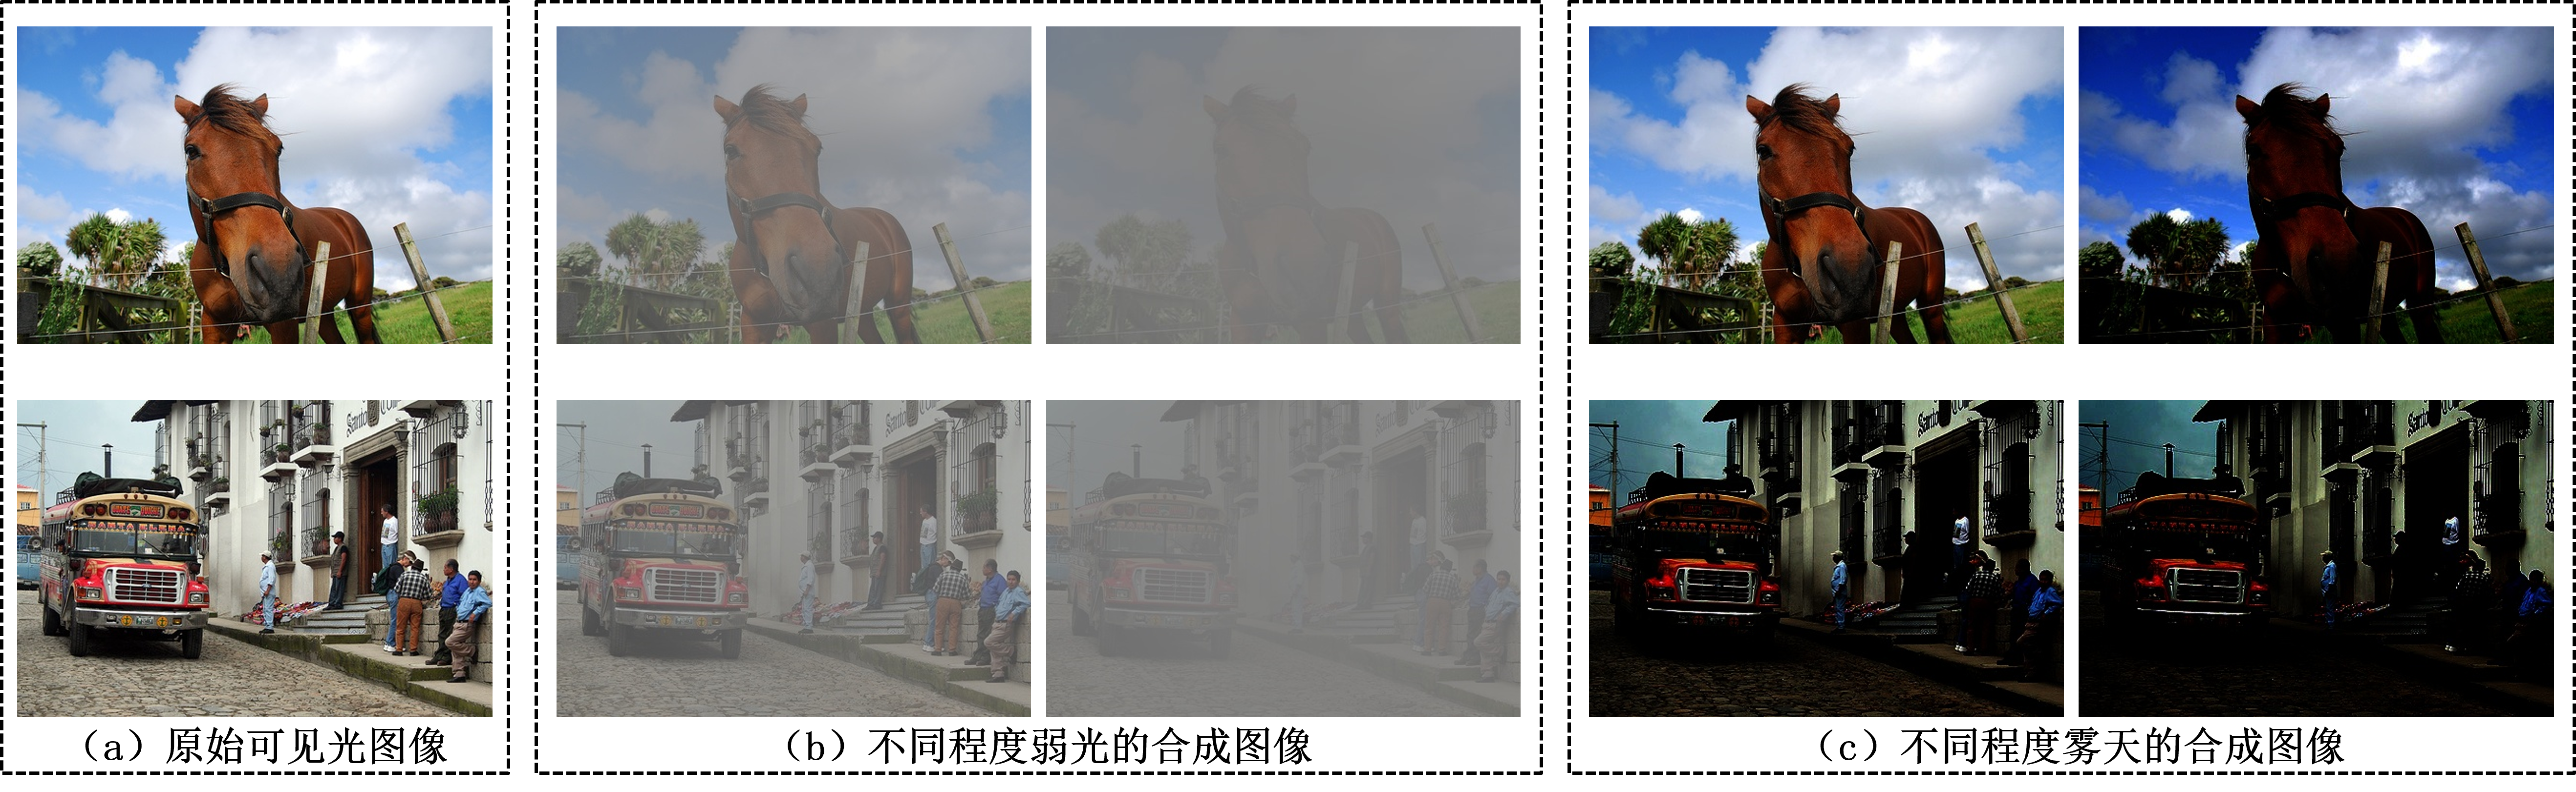
\includegraphics[width=16cm]{chapter4/9.png}
    \caption{\label{fig:ch4_9}原始图像与合成雾天、弱光退化图像对比示例}
\end{figure}

\textbf{2. 分阶段训练策略}

尽管端到端训练能够理论上实现全局最优,但在实践中,直接联合训练未经初始化的DPFE与YOLOv3往往会导致训练不稳定。

实验发现,由于BPW滤波器具有极强的像素映射能力,若缺乏有效的初始约束,增强器倾向于过度拉伸对比度,导致图像快速过曝、色调严重漂移(如\autoref{fig:ch4_10}所示),进而
使检测器难以提取有效的梯度特征,最终导致模型梯度爆炸或无法收敛。
\begin{figure}[htbp]
    \centering
    \includegraphics[width=15cm]{chapter4/10.png}
    \caption{\label{fig:ch4_10}缺乏初始约束时增强器输出图像随训练迭代发生退化的过程可视化}
\end{figure}

为了解决这一问题,我们采用“预热-联合”的分阶段训练策略,具体包含以下两个阶段:

\textbf{第一阶段:增强器预热}。
在训练的前20个轮次中,我们冻结后端YOLOv3检测器的所有参数,仅利用图像增强损失$L_{enh}$对前端DPFE进行优化。
此阶段旨在让增强器在无检测任务干扰的情况下,优先学习基本的图像恢复能力(如去雾、亮度校正),将退化图像恢复至正常的像素分布范围,从而为后续联合训练提供一个稳定的初始状态。

\textbf{第二阶段:联合微调}。
预热结束后,解冻检测器参数,将DPFE与YOLOv3进行端到端的联合训练。
此时,总损失函数包含了检测损失与增强损失,使增强器能够根据检测任务的反馈(如哪些区域的特征对检测更重要)进一步微调细节恢复策略,实现视觉质量与感知能力的双重提升。

\textbf{3. 损失函数设计}

为了在提升检测精度的同时保证图像的视觉质量,防止再次出现过曝或色彩失真,我们设计了由检测损失和增强损失组成的混合损失函数:
\begin{equation}
L_{total} = L_{det} + \lambda_{enh}L_{enh}
\end{equation}
其中,$\lambda_{enh}$为平衡系数(实验设置为$1.0$)。

\textbf{(1)检测损失}

检测部分沿用YOLOv3的原生损失函数,包含边界框坐标回归损失、置信度损失以及分类损失。这部分损失直接驱动模型学习目标的定位与识别。

\textbf{(2)增强损失}

引入增强损失的核心目的是对DPFE的输出施加约束,防止增强器生成非自然的图像。该损失由重建损失、结构相似性损失、色彩一致性损失和感知损失四部分加权组成:
\begin{equation}
L_{enh} = \lambda_{rec}L_{rec} + \lambda_{ssim}L_{ssim} + \lambda_{color}L_{color} + \lambda_{per}L_{per}
\end{equation}
实验中设置$\lambda_{rec}=1.0$,$\lambda_{ssim}=1.0$,$\lambda_{color}=1.0$,$\lambda_{per}=0.5$。

\begin{itemize}
    \item \textbf{重建损失$L_{rec}$}:采用平滑$L_1$损失(Smooth $L_1$ Loss)来约束增强图像$I_{enh}$与清晰参考图像$I_{gt}$之间的像素级差异。相较于均方差损失函数,
    平滑$L_1$损失对异常值不敏感,更有利于训练初期的收敛。
    \item \textbf{结构相似性损失 $L_{ssim}$}:为了保持图像的结构信息与纹理细节,避免增强过程中的结构扭曲,我们引入多尺度结构相似性(Multi-Scale Structural Similarity,MS-SSIM)损失作为约束。
    \item \textbf{色彩一致性损失 $L_{color}$}:
        尽管亮度增强能改善可见性,但往往伴随着严重的色彩失真。考虑到RGB空间中的欧氏距离无法有效反映人眼感知的色彩畸变\cite{color_loss_ref},我们引入基于余弦相似度的色彩一致性损失。
        我们强制增强图像的像素色彩向量与原始清晰图像的色彩分布保持一致,从而在去除退化的同时“注入”正确的色彩信息。其形式化定义为:
        \begin{equation}
            L_{color} = 1 - \frac{1}{N_{pix}} \sum_{i} \frac{I_{enh}^{(i)} \cdot I_{gt}^{(i)}}{\|I_{enh}^{(i)}\|_2 \|I_{gt}^{(i)}\|_2}
        \end{equation}
        其中,$I^{(i)}$表示第$i$个像素的RGB向量。
    \item \textbf{感知损失 $L_{per}$}:
    为了提升图像在特征层面的语义一致性,我们引入基于对比学习思想的感知损失。
    利用预训练的VGG-16网络作为特征提取器$\phi(\cdot)$,提取增强图像$I_{enh}$、清晰图像$I_{gt}$(正样本)以及退化图像$I_{deg}$(负样本)的中间层特征。
    该损失通过三元组损失的形式,强迫增强图像的特征表示在特征空间中尽可能靠近正样本,同时远离负样本:
    \begin{equation}
        L_{per} = \max\left(0, \|\phi(I_{enh}) - \phi(I_{gt})\|_1 - \|\phi(I_{enh}) - \phi(I_{deg})\|_1 + m\right)
    \end{equation}
    其中$m$为边界阈值。这使得增强图像不仅在像素上逼近真值,更在感知语义上恢复了清晰图像的特征分布。
\end{itemize}

\subsection{自适应增强的可视化分析}
\label{subsec:ch4_2_4}
为深入理解双渐进滤波器(DPFE)的内部工作机制,验证其渐进增强策略的有效性,本节对DPFE在弱光和雾天两种典型退化场景下的处理过程进行可视化分析。
通过观察各级双流滤波块(DFB)中贝塞尔像素级滤波器(BPW)的映射曲线、基于局部滤波器(KBL)的增强效果、输入输出图像的变化以及门控权重的分配,我们可以
清晰追踪图像从退化状态逐步恢复到清晰域的完整过程。
\begin{figure}[htbp]
\centering
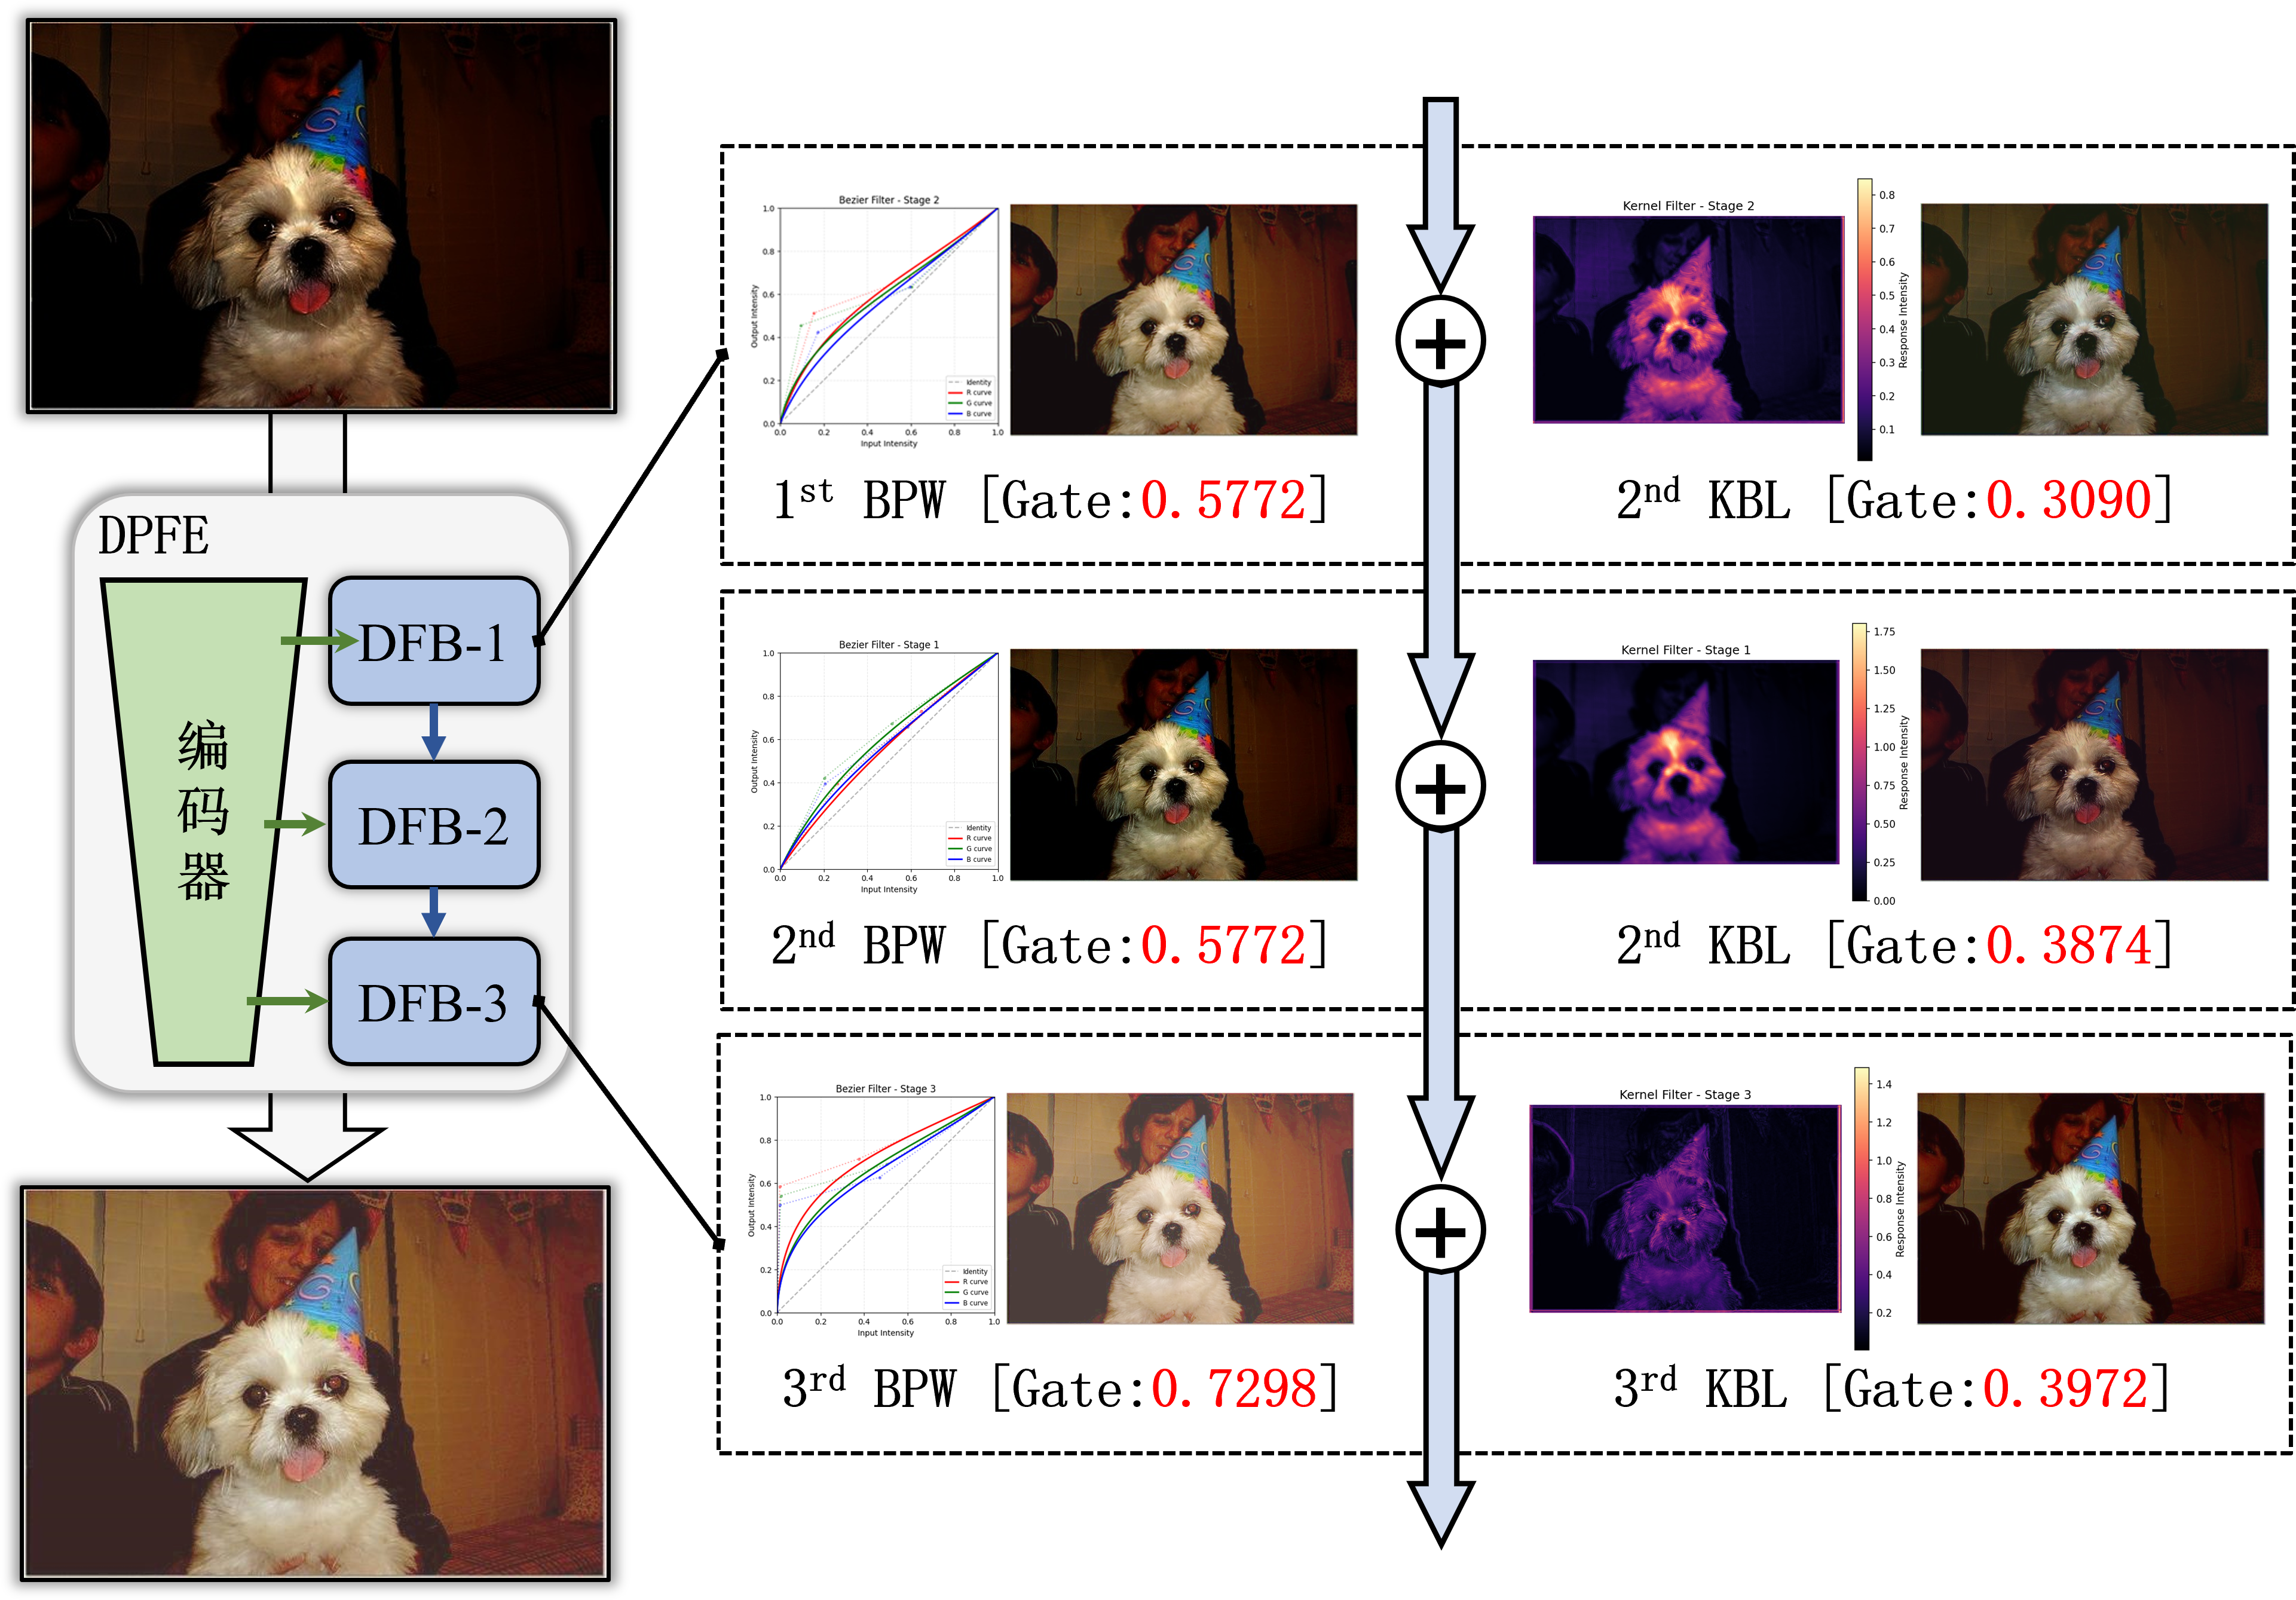
\includegraphics[width=15cm]{chapter4/11.png}
\caption{\label{fig:ch4_11}弱光场景下DPFE渐进增强过程可视化(三级DFB)}
\end{figure}

\autoref{fig:ch4_11}和\autoref{fig:ch4_12}分别展示了在弱光和雾天退化条件下,DPFE三级级联DFB的逐级增强可视化结果。
每个DFB的展示主要包括四部分内容:
(1) BPW支路输出图像 $I_{bpw}$:展示经过贝塞尔曲线全局映射后的结果,反映了色调、对比度的整体调整;
(2) KBL支路输出图像 $I_{kbl}$:展示经过局部卷积滤波后的结果,反映了边缘、纹理等细节的恢复;
(3) BPW滤波器在RGB三通道上的映射曲线:直观显示当前DFB所学习的像素级非线性变换函数;
(4) KBL滤波器增强前后的差分图($I_{kbl} - I_{in}$):用于突出局部细节的恢复效果。
此外,图中还标注了门控网络预测的融合权重 $(\omega_{bpw}, \omega_{kbl})$,用以量化两条支路在最终融合中的重要性。
\begin{figure}[htbp]
\centering
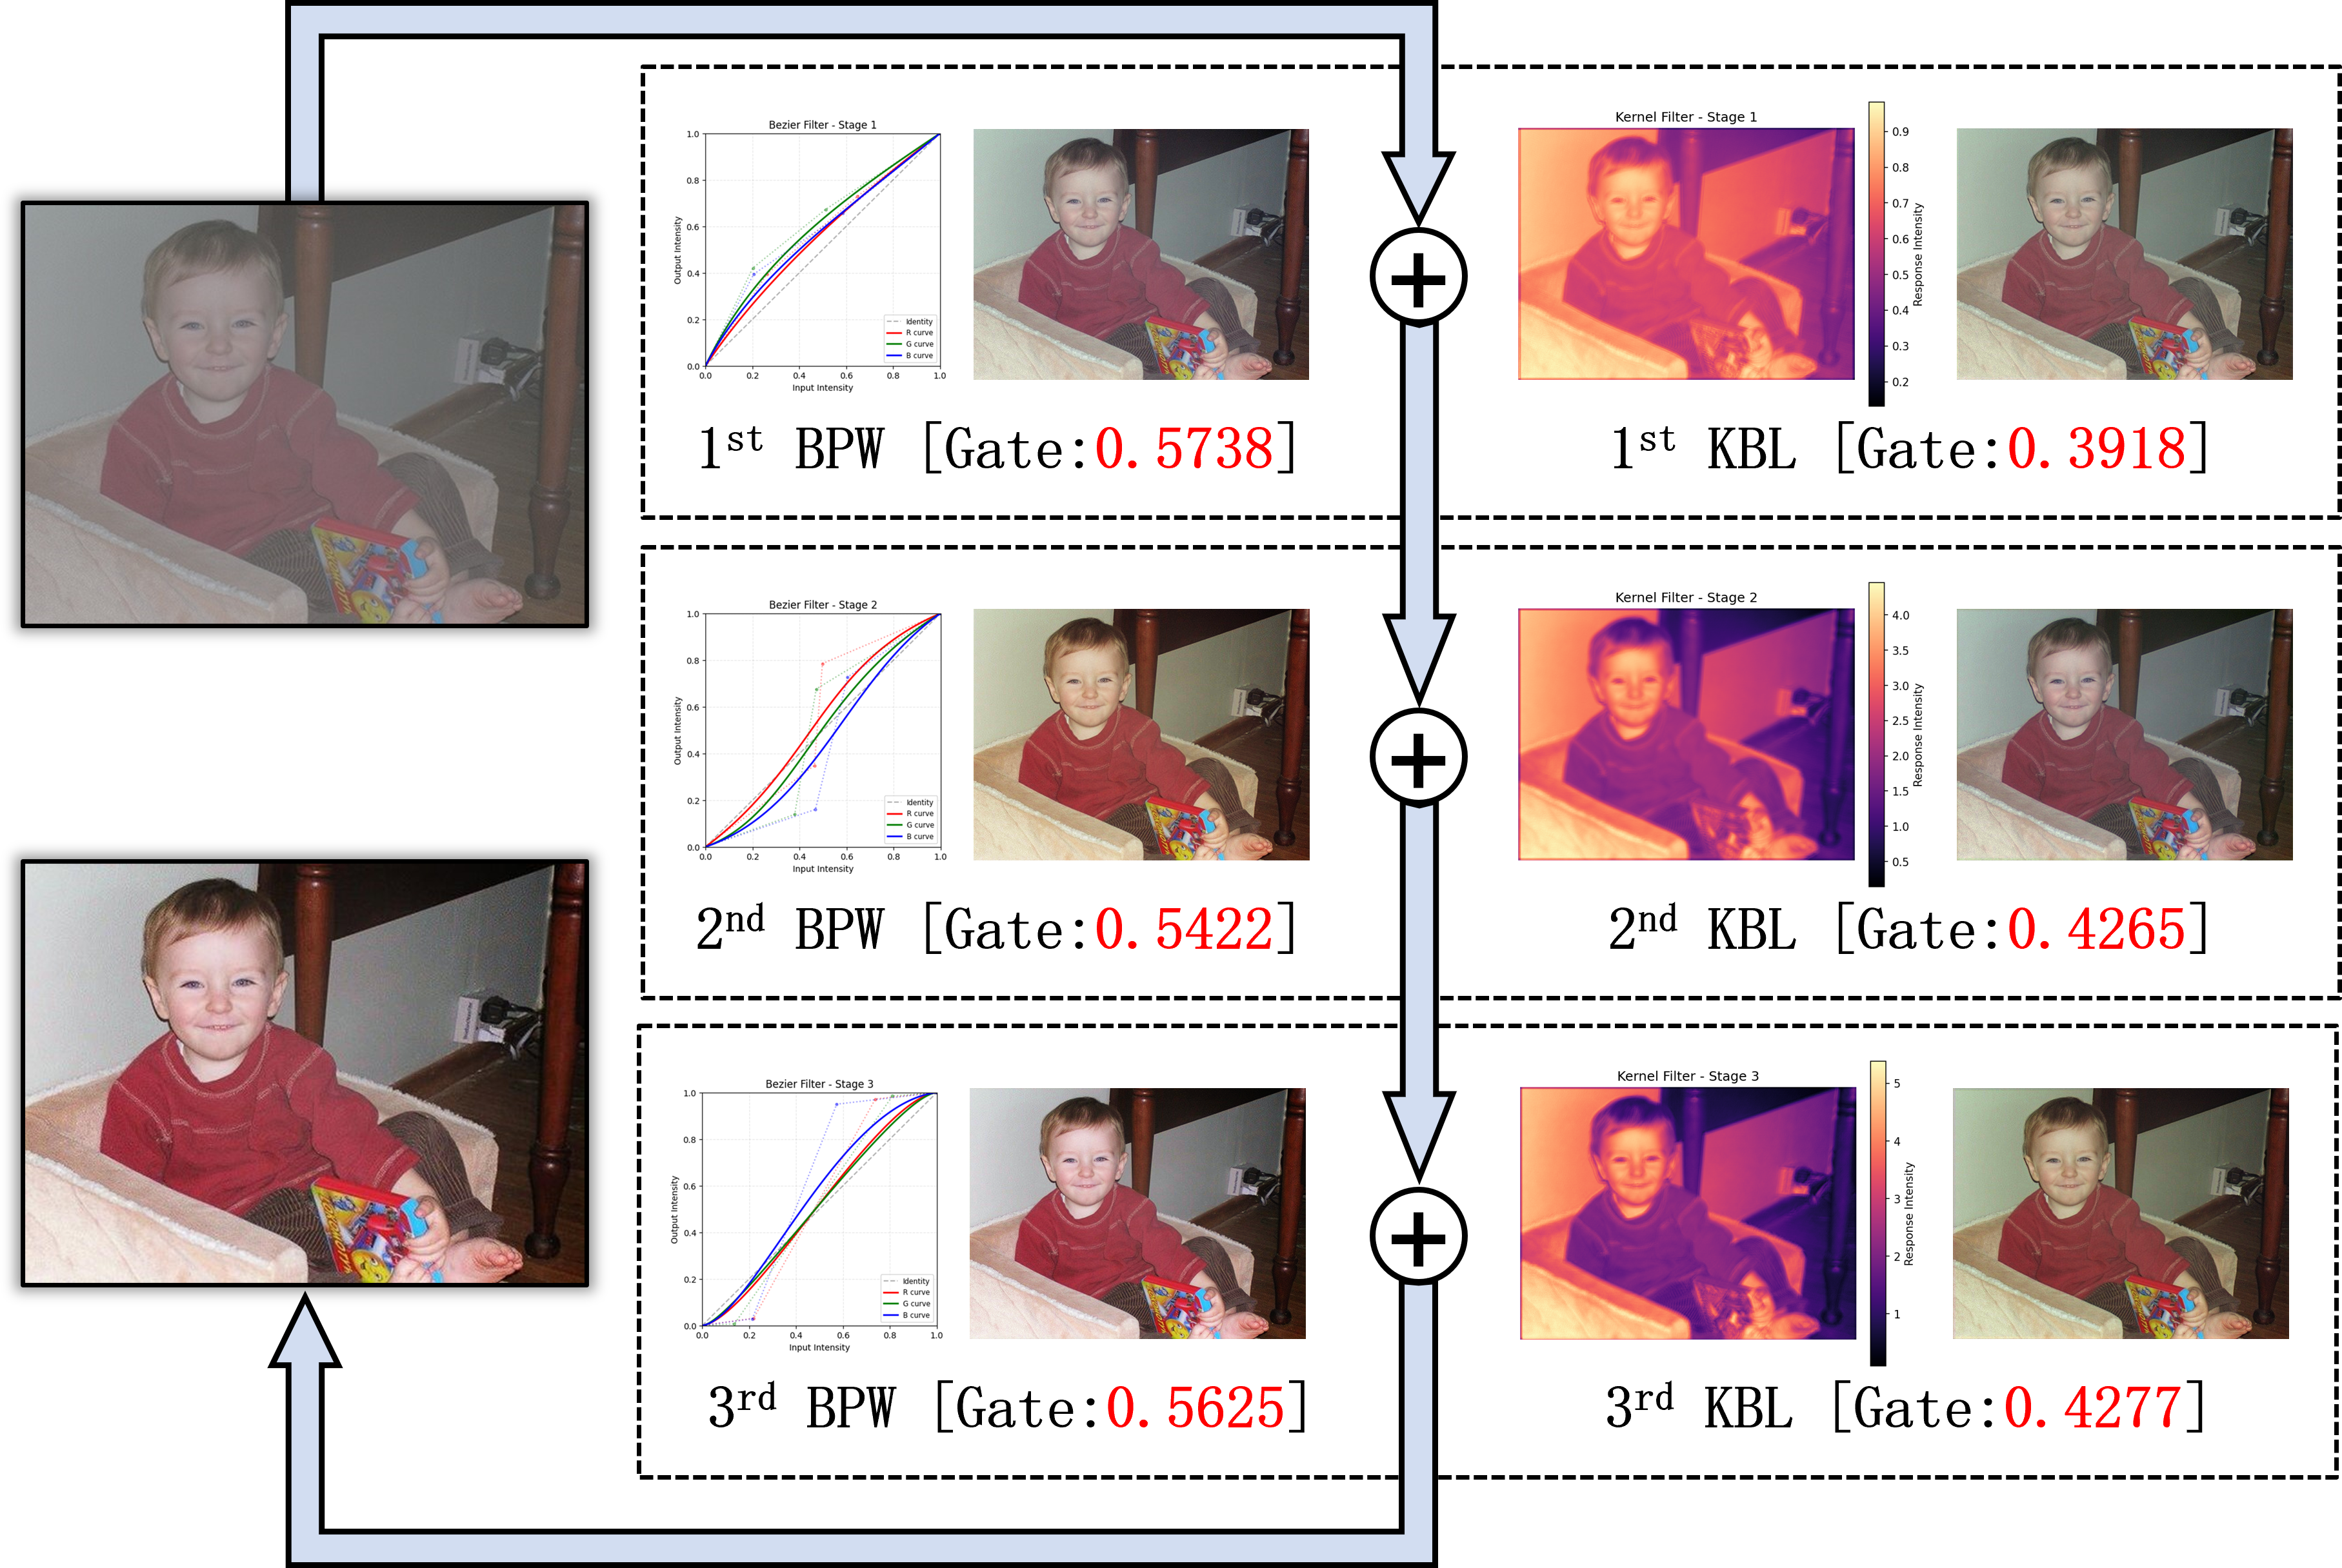
\includegraphics[width=15cm]{chapter4/12.png}
\caption{\label{fig:ch4_12}雾天场景下DPFE渐进增强过程可视化(三级DFB)}
\end{figure}

从可视化结果中可以观察到以下几个关键现象:

\textbf{1. 渐进增强的层次性体现}:在两种退化场景下,DPFE仅通过三级处理即展现出清晰的“由粗到细”的渐进增强特性。
对于DFB-1,BPW映射曲线接近线性恒等映射($y=x$),KBL差分图的幅值也相对较小,
这表明初始阶段增强器采取了一种保守策略,仅进行基础的、小幅度的全局校正与局部平滑,
旨在稳定地初始化恢复过程,避免早期过度增强引入失真。
进入DFB-2和DFB-3,BPW曲线开始呈现出明确的非线性形态:
在弱光场景中曲线明显上凸以提亮暗部,在雾天场景中则下凹以拉伸全局对比度。
同时,KBL差分图的幅值与细节丰富度显著增加,显示模型在后期阶段进行了更强力的局部结构修复与边缘增强。

\textbf{2. 退化模式的自适应处理}:DPFE能够根据不同的退化类型自适应地调整其增强策略的侧重点与演进路径。
在弱光场景中,BPW的增强强度(曲线上凸程度)在DFB-2和DFB-3阶段持续显著增加,成为主导的恢复力量,这与提升整体亮度以对抗光照不足的物理直觉一致。
而在雾天场景中,KBL的局部增强作用相对更为突出,其差分图在DFB-2中显示出比弱光场景更丰富的边缘恢复信号,表明网络更早、更主动地致力于消除雾霾导致的模糊并恢复纹理细节。

\textbf{3. 门控权重的动态决策分析}:门控权重的数值(可视化示例中的具体值见\autoref{tab:gate_weights})为上述自适应行为提供了直接的量化证据。
这些权重由Sigmoid函数独立产生,其和为模型对当前样本所需总增强强度的动态评估。

\begin{table}[htbp]
    \centering
    \caption{可视化示例中弱光与雾天样本在各DFB的门控权重 $(\omega_{bpw}, \omega_{kbl})$}
    \label{tab:gate_weights}
    \begin{tabular}{cccc}
        \toprule
        \textbf{场景} & \textbf{DFB-1} & \textbf{DFB-2} & \textbf{DFB-3} \\
        \midrule
        弱光 & (0.5772, 0.3874) & (0.6091, 0.3090) & (0.7298, 0.3972) \\
        雾天 & (0.5738, 0.3918) & (0.5422, 0.4265) & (0.6215, 0.3268) \\
        \bottomrule
    \end{tabular}
\end{table}

分析该示例的权重数据可知:在弱光场景下,全局校正路径的权重 $\omega_{bpw}$ 从0.5772持续上升至0.7298,占据越来越主导的地位。
而在雾天场景下,$\omega_{bpw}$ 的上升相对缓和,且在DFB-2中局部路径权重 $\omega_{kbl}$ 达到较高的0.4265,
体现了对局部恢复的阶段性侧重。
两个场景在末级DFB的权重总和均大于1(弱光1.127,雾天0.9483),
表明网络判定弱光样本需要更强的整体增强力度。
这种非归一化的、动态的权重分配机制,是DPFE实现针对不同退化类型与程度进行精细化、自适应增强的核心。

\textbf{4. 局部细节的递进恢复}:通过并行观察三级KBL输出图像及其差分图,可以清晰看到局部细节的恢复是一个递进过程。
KBL的输出从最初的轻微平滑/去噪,逐步过渡到在DFB-3中恢复出精细的物体轮廓和表面纹理,
其差分图也由大面积的低频调整演变为聚焦于边缘的高频增强。

上述可视化分析充分证实了DPFE设计的合理性和有效性。
该方法通过双路并行的全局像素映射与局部结构滤波,
并结合可学习的门控机制,构建了一种由粗到细的渐进式自适应增强过程,
从而稳定、高效地生成视觉质量高、细节丰富、色彩自然的清晰图像,为下游检测与跟踪任务提供了可靠的视觉前端。
\section{跨域自适应检测与跟踪推理框架}
\label{sec:ch4_3}
在解决了跨域环境下的特征退化与前端检测适配问题后,构建高效跨域多目标跟踪系统的最后一步是实现各功能模块的系统级集成。
本节旨在将训练完毕的前端自适应增强模块(DPFE)与目标检测器、后端双图协同关联模块(DGCTracker)进行有机融合,形成统一的推理闭环。

如\autoref{fig:ch4_13}所示,本节提出的跨域自适应多目标检测与跟踪系统采用了模块化级联架构,
构建了一条从原始视频输入到轨迹输出的完整推理管线。
该管线由三个功能解耦的核心模块串行构成:前端的双渐进滤波增强器(DPFE)、中端的通用目标检测器(如YOLOv3)以及后端的双图协同跟踪器(DGCTracker)。
各模块协同工作,将复杂的跨域跟踪任务分解为“图像域恢复—清晰域检测—时空域关联”三个递进的处理阶段。
\begin{figure}[htbp]
    \centering
    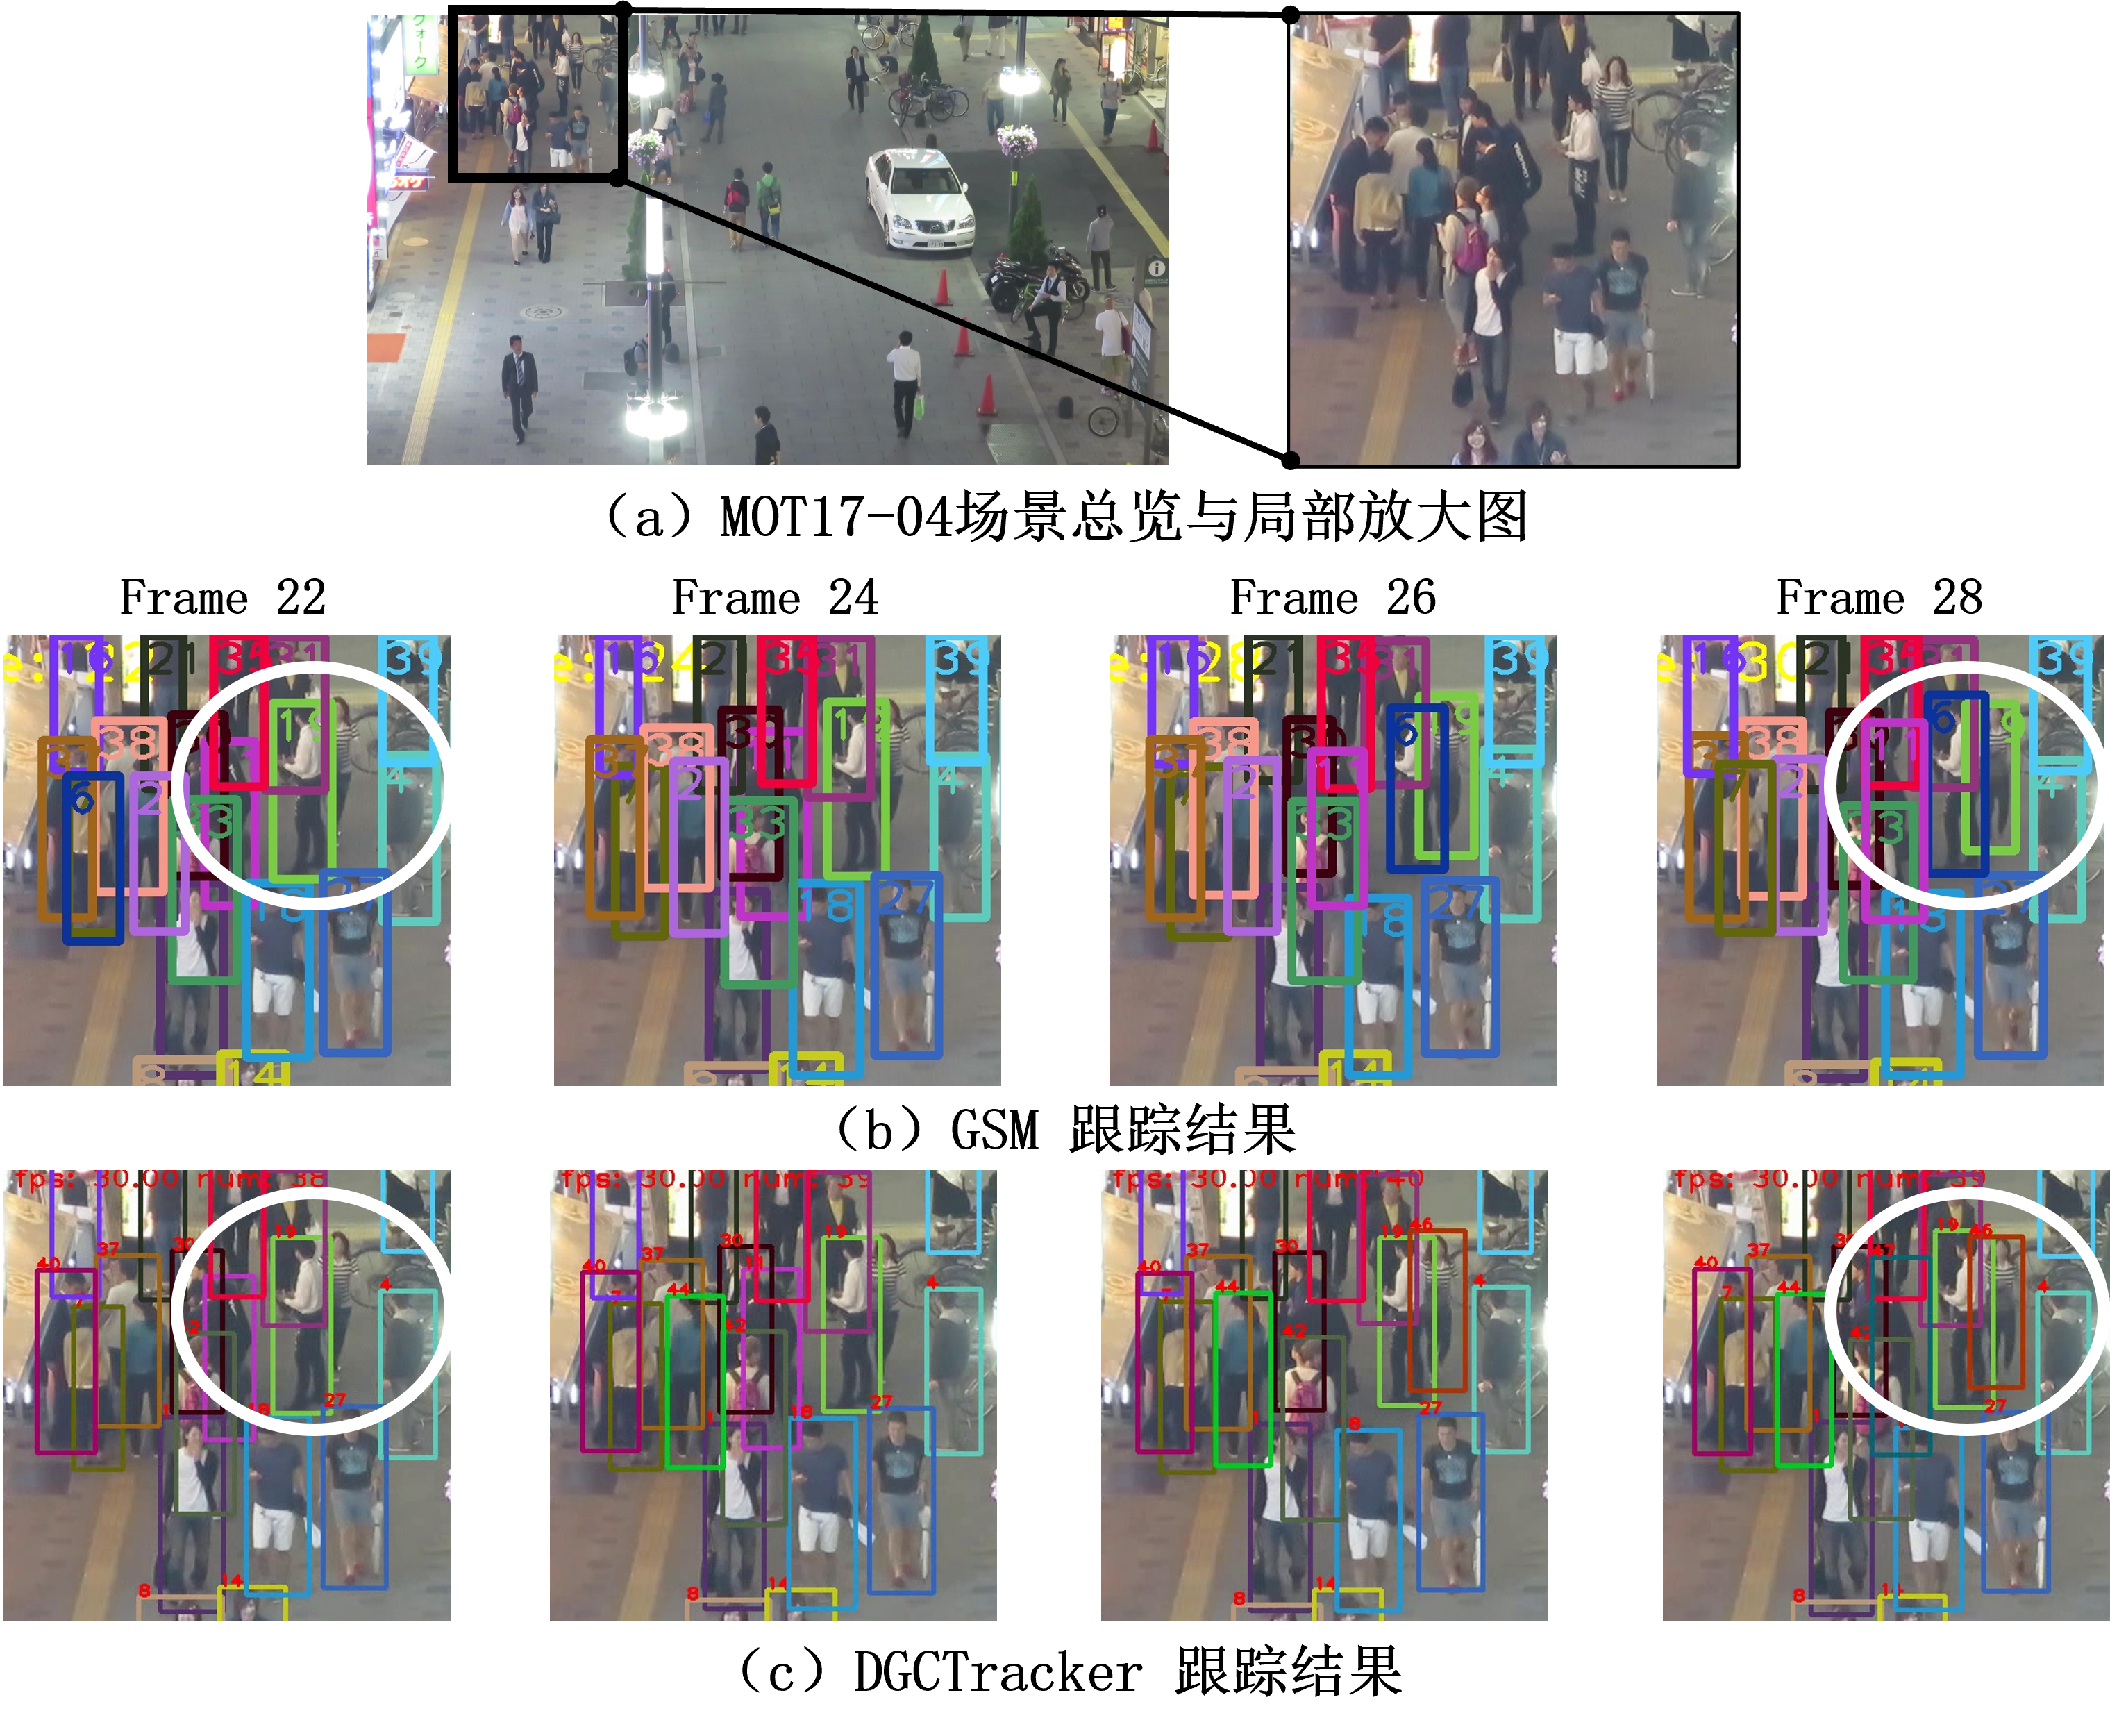
\includegraphics[width=15cm]{chapter4/13.png}
    \caption{\label{fig:ch4_13}跨域自适应多目标检测与跟踪系统推理管线}
\end{figure}

整个推理过程包含以下三个核心阶段:

\textbf{1. 图像域自适应恢复}:
系统的输入为连续的恶劣环境视频序列。这些退化帧首先被送入训练好的双渐进滤波增强器(DPFE)。该模块以“逐帧”在线处理的方式,将恶劣图像映射到清晰域,输出色彩自然、对比度高的视频流,从而在输入端消除环境干扰。

\textbf{2. 清晰域目标检测}:
增强后的视频流随即被送入目标检测模块。由于输入图像的质量已恢复至接近源域(清晰训练集)分布,检测器能够有效避免因光照不足或模糊导致的漏检问题。
在这一阶段,检测器能够生成清晰域下的检测集合$\mathcal{D}$。

\textbf{3. 时空域轨迹关联}:
最后,高质量的检测结果被传入后端的DGCTracker。
基于第三章提出的稀疏双图模型,跟踪器综合利用检测目标的空间位置信息与清晰的表观特征,对跨帧目标间的关联关系进行建模与推理,
并通过最优匹配策略完成目标身份分配,最终输出 ID 连续、身份稳定的轨迹集合$\mathcal{L}$,
从而完成完成跨域跟踪任务。

通过上述三个阶段的级联协作,本节构建的跨域自适应检测与跟踪推理框架在系统层面完成了从退化输入到稳定轨迹输出的闭环设计。
该框架在实际应用中对恶劣环境的适应能力及其整体运行效率,是衡量系统实用价值的关键因素。
下一节将通过一系列定量实验,从跨域跟踪的鲁棒性、系统参数量与实时性等方面,进行全面评估与分析。
\section{实验结果与讨论}
\label{sec:ch4_4}
为全面验证本章所构建的跨域自适应检测与跟踪推理框架的有效性与优越性,本节将展开系统性的实验评估与深入讨论。
评估工作主要围绕两大核心目标展开:
其一,验证所提出的自适应增强方法在跨域目标检测任务中的性能,确认其能否有效缓解视觉退化并超越现有先进方法;
其二,评估集成了增强、检测、跟踪模块的完整系统,在恶劣环境下的跟踪鲁棒性、实时处理能力以及工程部署潜力。
通过定性与定量相结合的分析,旨在从算法精度和系统工程两个维度,为整个框架的实用价值提供坚实依据。

本节内容组织如下:
\ref{subsec:ch4_4_1}小节将详细介绍实验所需的数据集、评价指标与关键实现细节;
\ref{subsec:ch4_4_2}小节将展示并分析所提方法在弱光与雾天场景下的跨域检测性能;
\ref{subsec:ch4_4_3}小节通过详尽的消融实验,剖析自适应增强模块中各个核心组件的贡献;
\ref{subsec:ch4_4_4} 节通过在多目标跟踪基准上引入合成退化,评估前端增强对维持系统跟踪稳定性的关键作用;
最后,\ref{subsec:ch4_4_5}小节将从参数量、推理速度以及架构可扩展性等方面,综合分析系统的工程效能与部署优势。
\subsection{实验条件设置}
\label{subsec:ch4_4_1}
为系统验证本章所提方法的有效性,本小节将详细阐述实验所需的数据集、评价指标与关键实现细节。
实验主要分为两部分:跨域目标检测性能验证与跨域多目标跟踪鲁棒性评估。前者在标准跨域检测基准上进行,后者则在多目标跟踪数据集上通过合成退化构建跨域场景进行验证。

\textbf{1. 跨域目标检测实验设置}

\textbf{数据集}:检测实验旨在评估方法对合成与真实退化的适应能力,涉及以下数据集(各数据集的详细介绍见\ref{subsec:ch2_3_2}节):
\begin{itemize}
    \item \textbf{清晰源域数据集(VOC\_norm)}:采用PASCAL VOC 2007测试集(4952张图像)作为清晰条件下的性能基准。
    \item \textbf{合成退化测试集(VOC\_dark / VOC\_fog)}:为在可控条件下进行公平对比,我们采用IA-YOLO工作开源的标准合成退化数据集。该数据集通过对PASCAL VOC 2007测试集图像分别应用其定义的弱光/雾天退化模型而生成,记为VOC\_dark与VOC\_fog。
    \item \textbf{真实退化测试集(ExDark / RTTS)}:使用真实场景下的弱光数据集ExDark与雾天数据集RTTS作为测试集,进一步验证方法在真实跨域场景中的泛化能力。
\end{itemize}

\textbf{评价指标}:统一采用\ref{subsec:ch2_3_2}节中介绍的$\text{mAP@0.5}$作为评价指标,用于衡量不同方法在清晰域及跨域退化条件下的检测精度。

\textbf{实现与训练细节}:所有跨域检测模型均在NVIDIA RTX 4090 GPU平台上进行训练与推理。YOLOv3检测器主干网络加载了在MS COCO数据集上预训练的权重,以加速收敛。
训练策略严格遵循\ref{subsec:ch4_2_3}节所述的分阶段训练策略:首先固定检测器权重,仅使用增强损失对DPFE模块进行20个轮次的预训练;
随后进行端到端联合微调。优化采用随机梯度下降(SGD),动量为0.937,权重衰减为5e-4。
初始学习率设为$1\times10^{-3}$,采用余弦退火策略降至$1\times10^{-5}$。
总训练轮数为80,批次大小设置为64。
针对不同的退化类型,我们分别训练了专用的模型权重,即使用弱光退化数据训练“弱光增强-检测”模型,使用雾天退化数据训练“雾天增强-检测”模型,以确保对特定退化模式的最优适应。

\textbf{2. 跨域多目标跟踪实验设置}

\textbf{数据集与退化合成}:由于现有公开数据集缺乏同一视频序列下“清晰-雾天-弱光”的成对标注数据,无法直接用于定量评估跨域跟踪性能的损失与恢复情况。
因此,跟踪实验沿用 \ref{subsec:ch3_4_1} 节的数据划分策略,即选取 MOT17 训练集中每个视频序列的最后 100 帧作为测试片段。为构建跨域评估场景,
我们利用\ref{subsec:ch4_2_3}节中定义的物理退化模型,为该测试集生成了对应的弱光与雾天退化版本(MOT17\_dark与MOT17\_fog)。该合成数据集用于评估跟踪系统在跨域条件下的鲁棒性。

\textbf{评价指标}:跟踪指标依旧与\ref{subsec:ch3_4_1}节保持一致,即HOTA、IDF1、MOTA等综合指标。

\textbf{系统推理配置}:跨域跟踪实验的核心目的是评估前端增强模块对整个跟踪链路的增益。因此,后端DGCTracker直接加载其在原始清晰MOT17数据集上训练好的最优权重,不针对恶劣数据进行重训练。
前端DPFE-YOLO则根据测试视频的退化类型,加载前述训练好的“弱光增强”或“雾天增强”的权重进行感知推理。

\subsection{跨域目标检测性能对比}
\label{subsec:ch4_4_2}
为了客观评估DPFE-YOLO在跨域退化场景下的性能,我们选取了当前领域具有代表性的先进模型进行横向对比。
对比基准包括原始YOLOv3\cite{yolov3}检测器、基于特征对齐的无监督域适应方法DA-YOLO\cite{dayolo}
以及基于可微图像处理的检测方法——IA-YOLO\cite{ia}、GDIP-YOLO\cite{gdip}、ERUP-YOLO\cite{erup}。
为保证对比的公平性,所有对比方法的检测主干网络均采用YOLOv3,并统一在弱光与雾天两种典型退化场景下进行评估。

\textbf{1. 弱光场景下的增强与检测性能}

弱光场景下的检测性能对比如\autoref{tab:lowlight_comparison}所示。
DPFE-YOLO在该场景下展现了显著的优势。
在真实弱光数据集ExDark上,其mAP达到57.32\%,远超ERUP-YOLO的48.43\%,领先幅度达8.89个百分点。
值得注意的是,基于特征对齐的DA-YOLO方法在此类极端退化下性能严重衰退,甚至不及未增强的YOLOv3,这凸显了在像素分布发生剧烈偏移时,仅在高维特征空间进行对齐的局限性。
\begin{table}[htbp]
  \centering
  \caption{弱光场景跨域目标检测性能对比 (mAP@0.5)}
  \label{tab:lowlight_comparison}
  \resizebox{0.9\linewidth}{!}{
  \begin{tabular}{cccccc}
    \toprule
    \textbf{Method} & \textbf{VOC\_norm (Clear)} $\uparrow$ & \textbf{VOC\_dark (Syn)} $\uparrow$ & \textbf{ExDark (Real)} $\uparrow$ \\
    \midrule
    YOLOv3          & 65.33 & 52.28 & 37.03 \\
    DA-YOLO         & 41.68 & 21.53 & 18.15 \\
    IA-YOLO         & 70.02 & 59.40 & 40.37 \\
    GDIP-YOLO       & 63.23 & 57.85 & 42.56 \\
    ERUP-YOLO       & 68.62 & 59.81 & 48.43 \\
    \textbf{DPFE-YOLO} & \textbf{84.23} & \textbf{81.29} & \textbf{57.32} \\
    \bottomrule
  \end{tabular}
  }
\end{table}

\autoref{fig:ch4_15}的定性对比清晰地展示了DPFE-YOLO在弱光处理上的关键优势。
ERUP-YOLO的增强结果存在明显的局部过曝现象,尤其是在路灯等高亮区域,这可能导致细节丢失并干扰检测。
而DPFE-YOLO的增强效果更为均衡自然,在整体提升亮度的同时,有效抑制了过曝,保留了丰富的纹理细节。
相应的检测结果显示,DPFE-YOLO对前方主要车辆的检测置信度达到0.94,高于ERUP-YOLO的结果。
\begin{figure}[htbp]
    \centering
    \includegraphics[width=12cm]{chapter4/15.png}
    \caption{\label{fig:ch4_15}真实弱光场景下DPFE-YOLO与ERUP-YOLO的定性对比}
\end{figure}

\textbf{2. 雾天场景下的增强与检测性能}

雾天场景下的跨域检测性能对比如\autoref{tab:foggy_comparison}所示。
定量结果表明,所提出的DPFE-YOLO在清晰域(VOC\_norm)、合成雾天域(VOC\_fog)及真实雾天域(RTTS)上均取得了最优性能。
具体而言,在最具挑战的真实雾天数据集RTTS上,DPFE-YOLO的mAP达到56.76\%,较其基线ERUP-YOLO(49.81\%)提升了6.95个百分点。
即使在合成雾天域VOC\_fog上,DPFE-YOLO也以81.80\%的mAP显著领先于ERUP-YOLO的74.09\%。
\begin{table}[htbp]
  \centering
  \caption{雾天场景跨域目标检测性能对比 (mAP@0.5)}
  \label{tab:foggy_comparison}
  \resizebox{0.9\linewidth}{!}{
  \begin{tabular}{cccccc}
    \toprule
    \textbf{Method} & \textbf{VOC\_norm (Clear)} $\uparrow$ & \textbf{VOC\_fog (Syn)} $\uparrow$ & \textbf{RTTS (Real)} $\uparrow$ \\
    \midrule
    YOLOv3          & 64.13 & 63.40 & 30.80 \\
    DA-YOLO         & 56.51 & 55.11 & 29.93 \\
    IA-YOLO         & 73.23 & 72.03 & 37.08 \\
    GDIP-YOLO       & 73.70 & 71.92 & 42.42 \\
    ERUP-YOLO       & 77.89 & 74.09 & 49.81 \\
    \textbf{DPFE-YOLO} & \textbf{82.47} & \textbf{81.80} & \textbf{56.76} \\
    \bottomrule
  \end{tabular}
  }
\end{table}

\autoref{fig:ch4_14}展示了DPFE-YOLO与ERUP-YOLO在真实雾天场景下的检测结果对比。
在视觉增强效果方面,本章方法所恢复的图像细节更为丰富,整体观感更为自然,有效避免了 ERUP-YOLO 在远处区域因过度去雾而产生的局部过曝现象。
在检测性能上,对于中近景的车辆与行人目标,DPFE-YOLO展现出更高的召回率与检测置信度,其生成的边界框也更为准确,这直接证明了渐进式增强策略在提升主要目标检测可靠性方面的优势。
\begin{figure}[htbp]
    \centering
    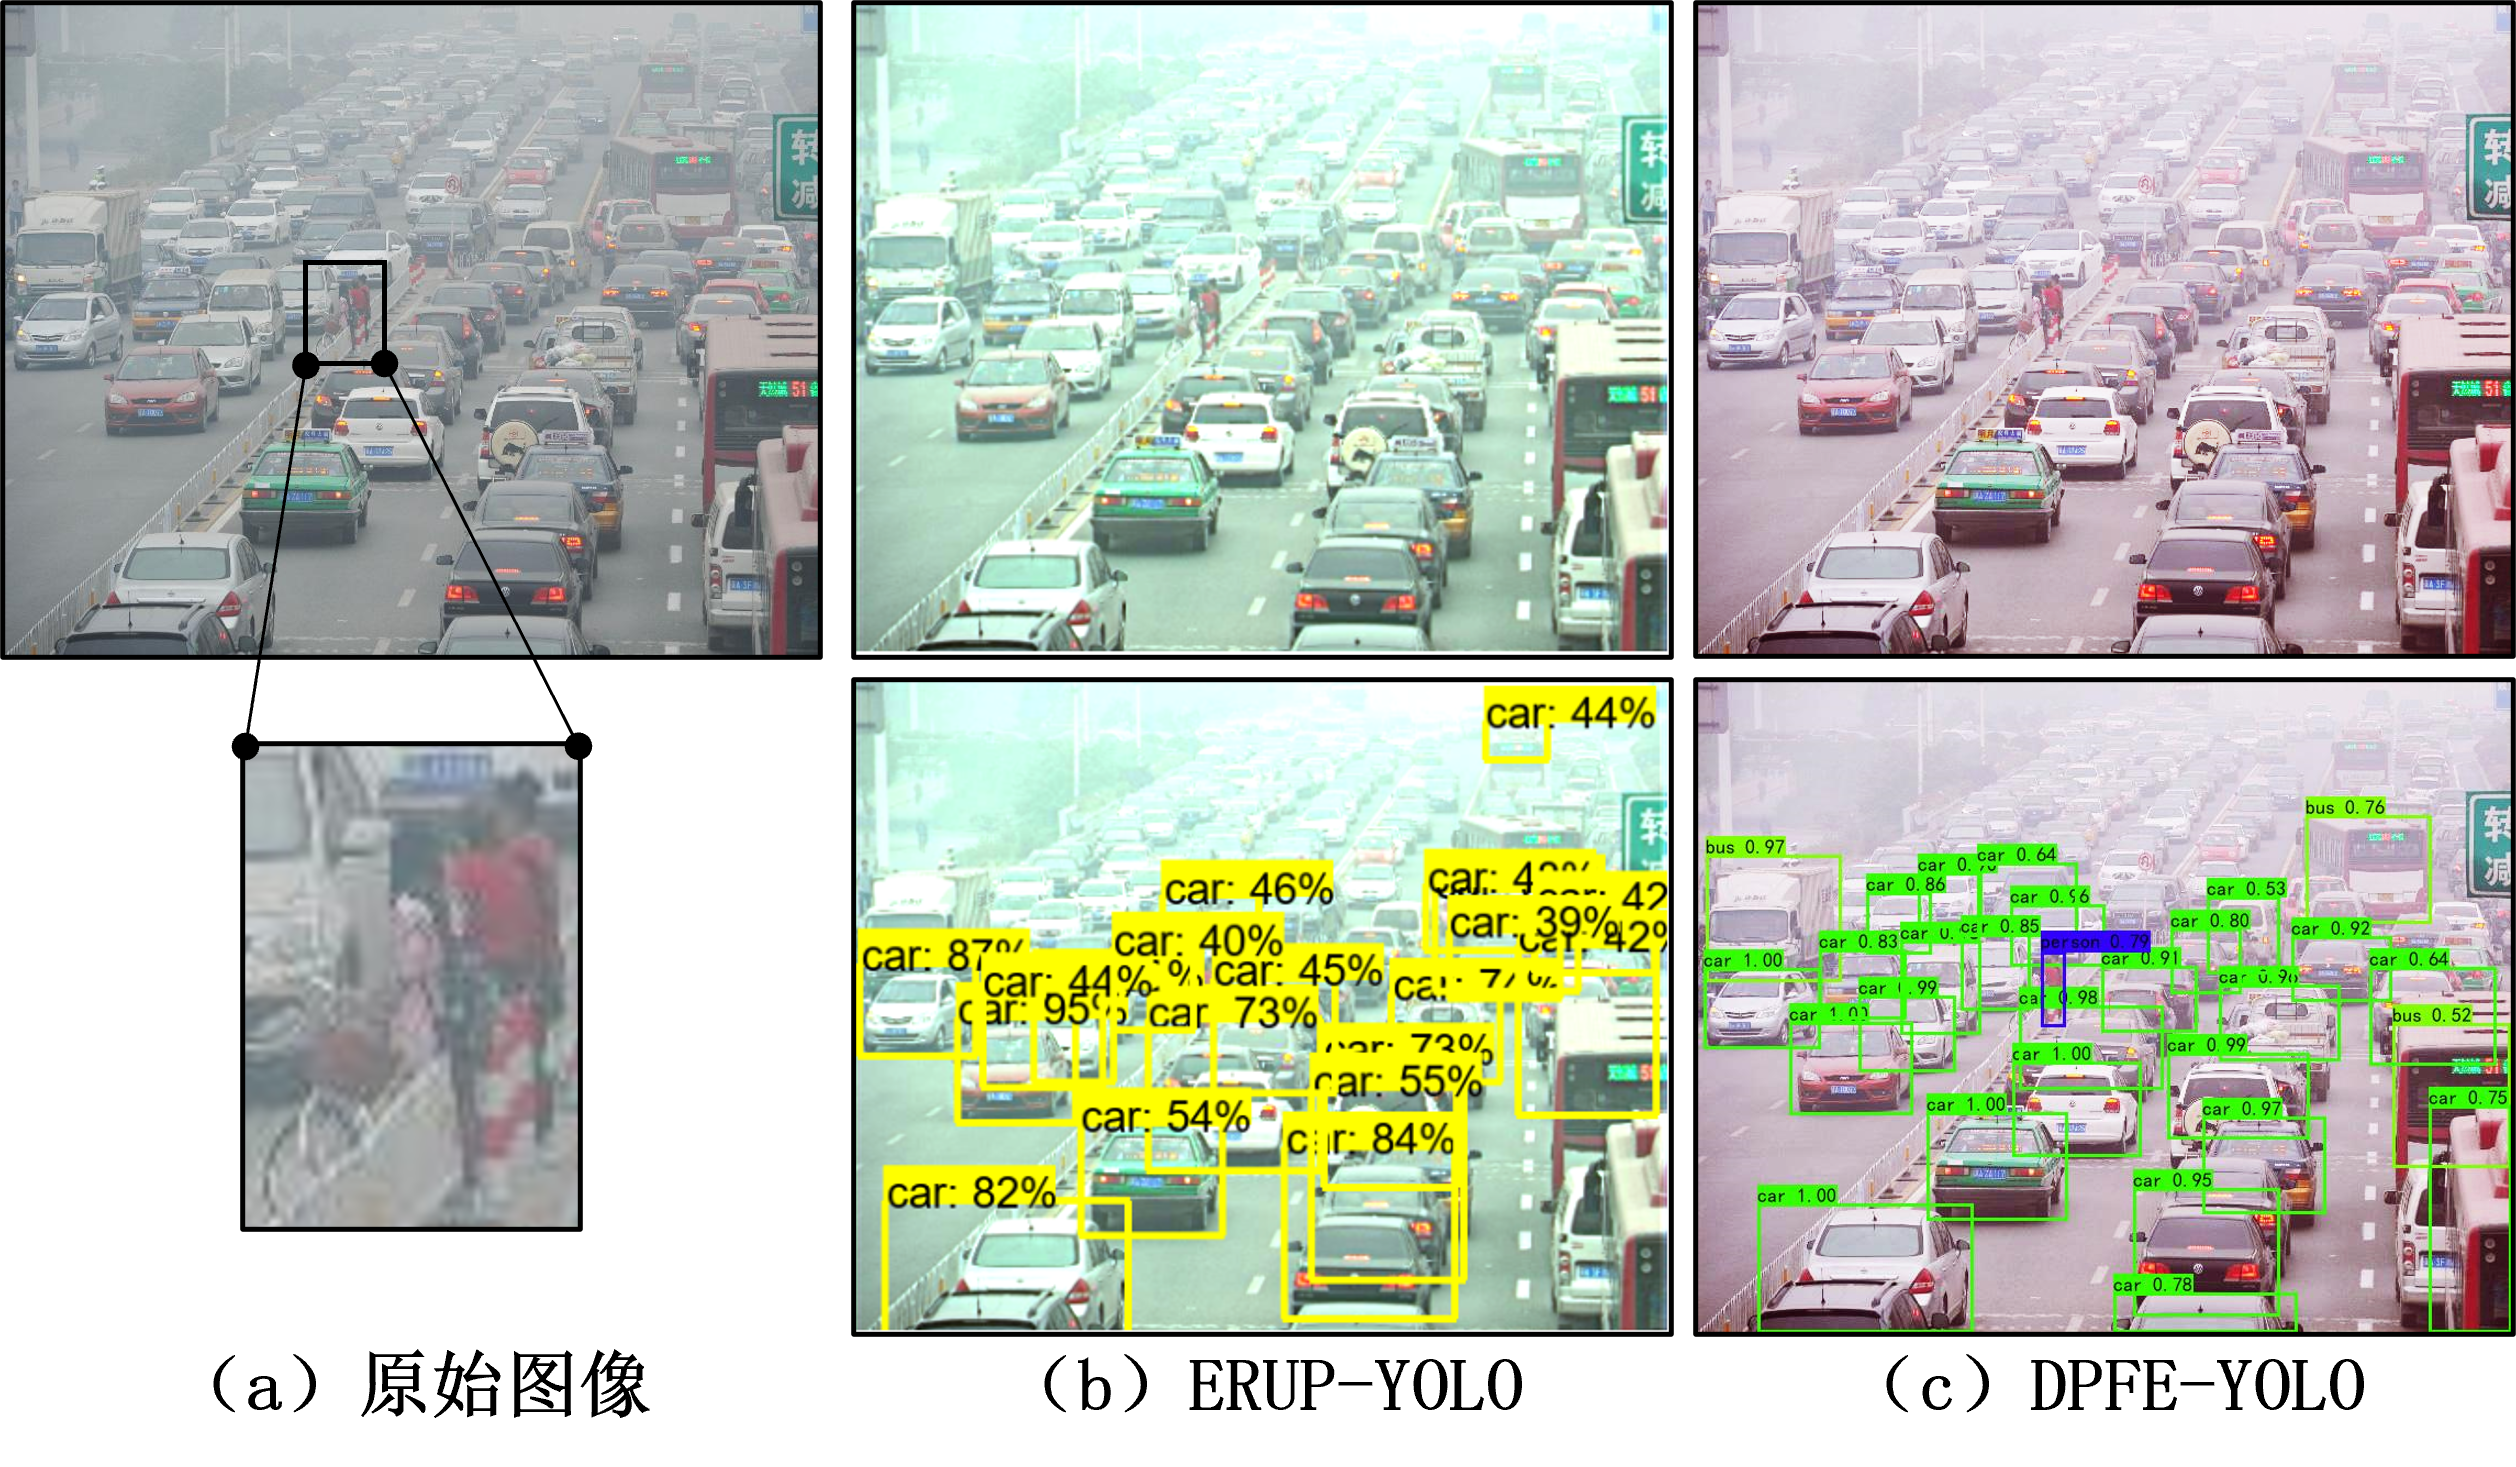
\includegraphics[width=15cm]{chapter4/14.png}
    \caption{\label{fig:ch4_14}真实雾天场景下DPFE-YOLO与ERUP-YOLO的定性对比}
\end{figure}

\textbf{3. 更多场景的可视化示例}

为了能够更加全面、直观地展示 DPFE-YOLO 在各类不同跨域场景下的增强与检测综合性能,
图\ref{fig:ch4_16}至图\ref{fig:ch4_19}分别提供了其在VOC\_dark(合成弱光)、ExDark(真实弱光)、VOC\_fog(合成雾天)、及RTTS(真实雾天)四个测试集上的处理结果可视化。

从图中可清晰观察到,DPFE模块能够有效恢复弱光下的暗部细节、消除雾天带来的朦胧感,并保持色彩的自然与一致性。
增强后的图像为后端检测器提供了显著更优的输入,从而在所有场景中均实现了更高的目标召回率、更少的漏检,以及整体更高的检测置信度。
这些直观的可视化结果进一步印证了所提方法在多样化真实跨域场景中具备稳定的增强性能与可靠的检测提升能力。
\begin{figure}[htbp]
    \centering
    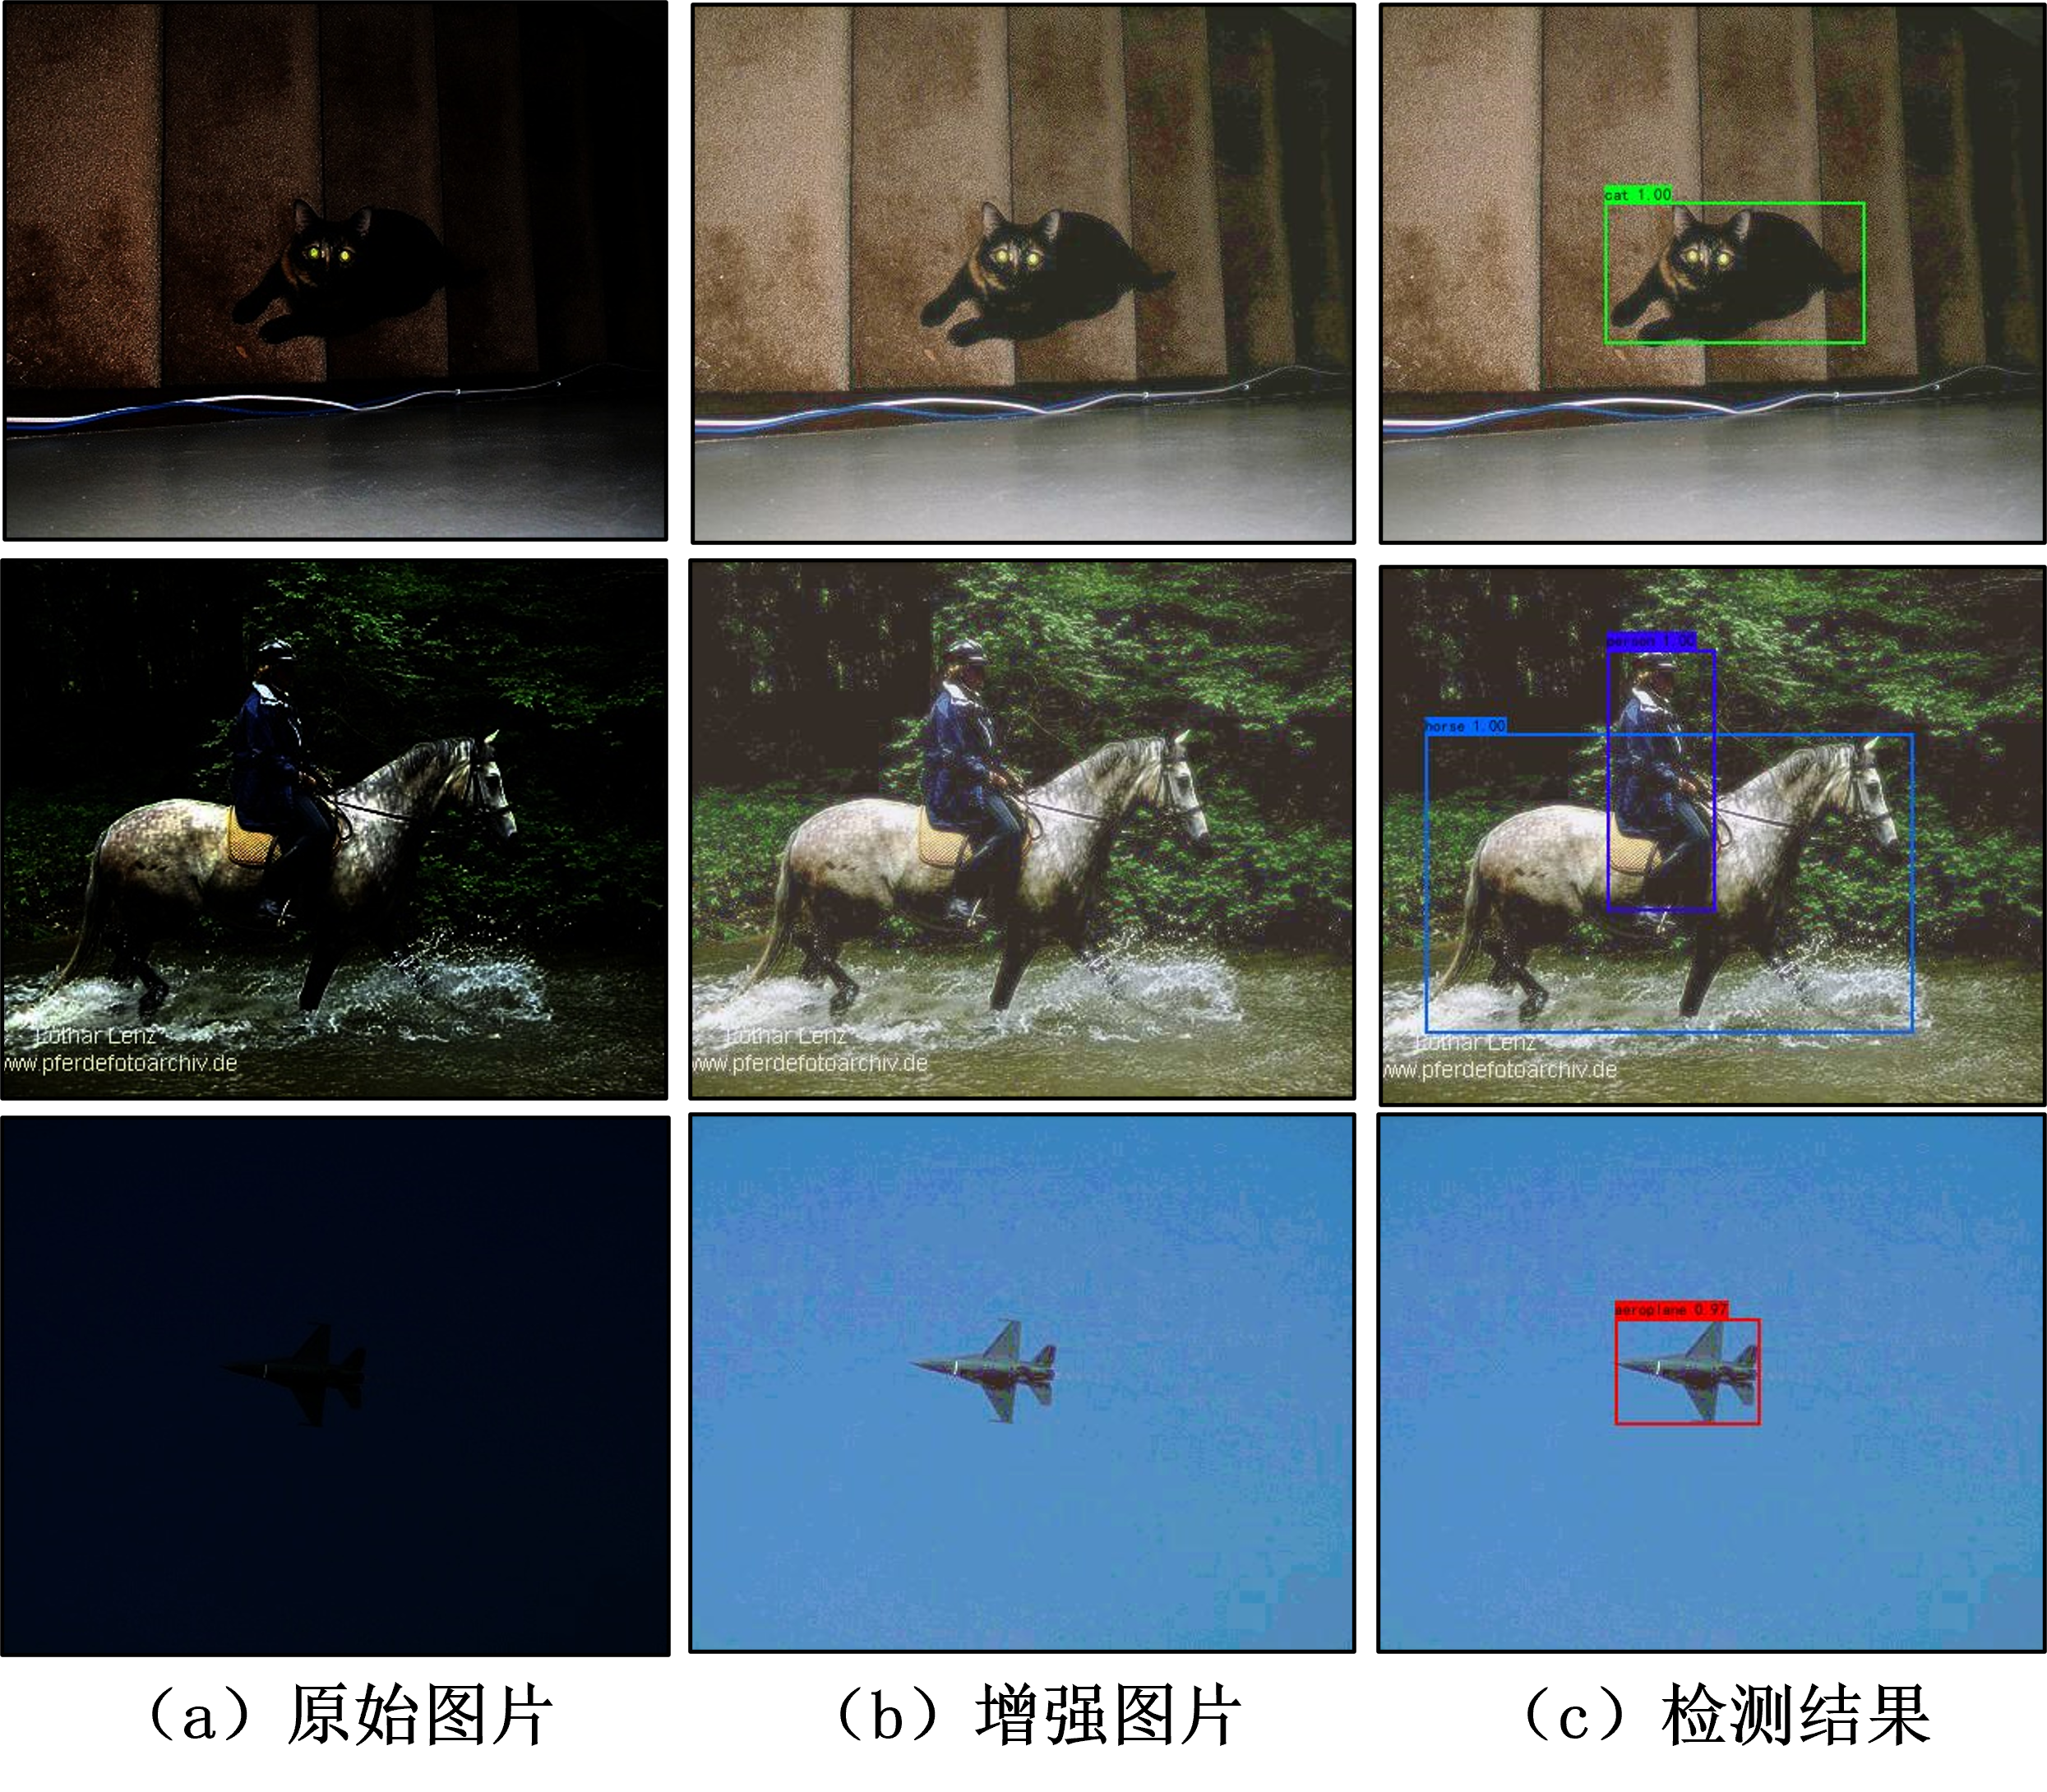
\includegraphics[width=13cm]{chapter4/16.png}
    \caption{\label{fig:ch4_16}DPFE-YOLO在VOC\_dark测试集上的部分增强与检测结果}
\end{figure}

\begin{figure}[htbp]
    \centering
    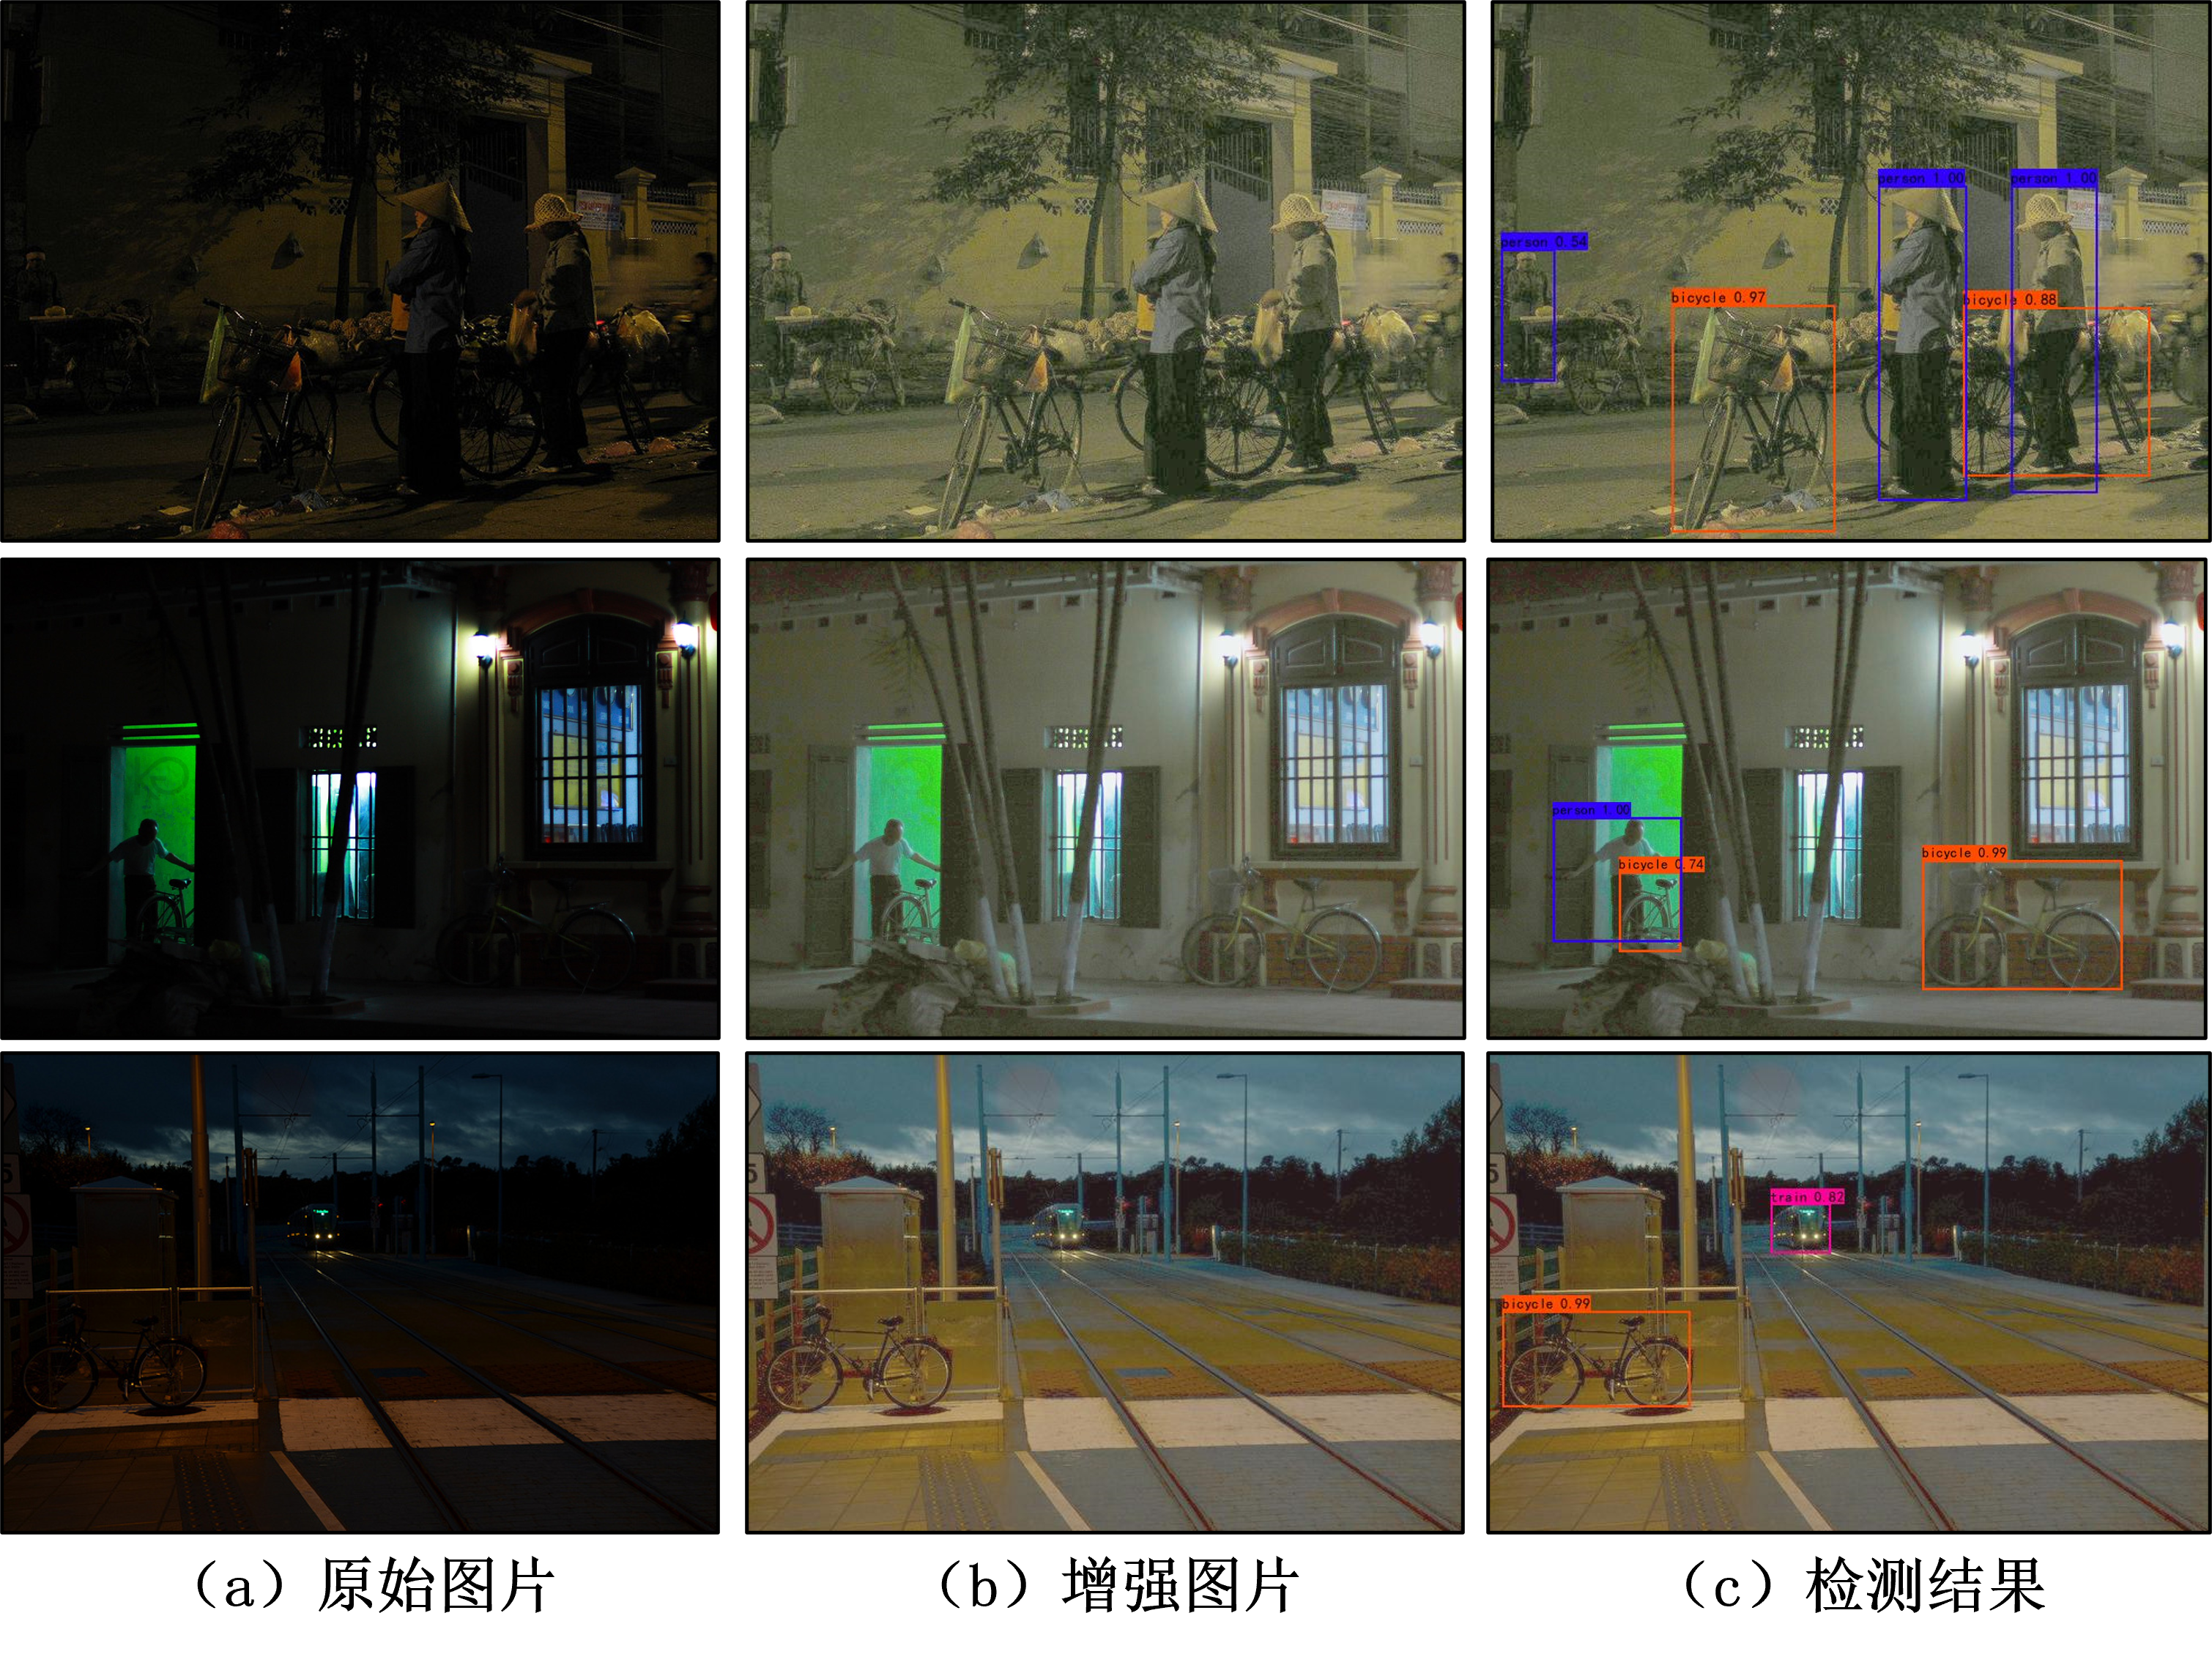
\includegraphics[width=13cm]{chapter4/17.png}
    \caption{\label{fig:ch4_17}DPFE-YOLO在ExDark测试集上的部分增强与检测结果}
\end{figure}

\begin{figure}[htbp]
    \centering
    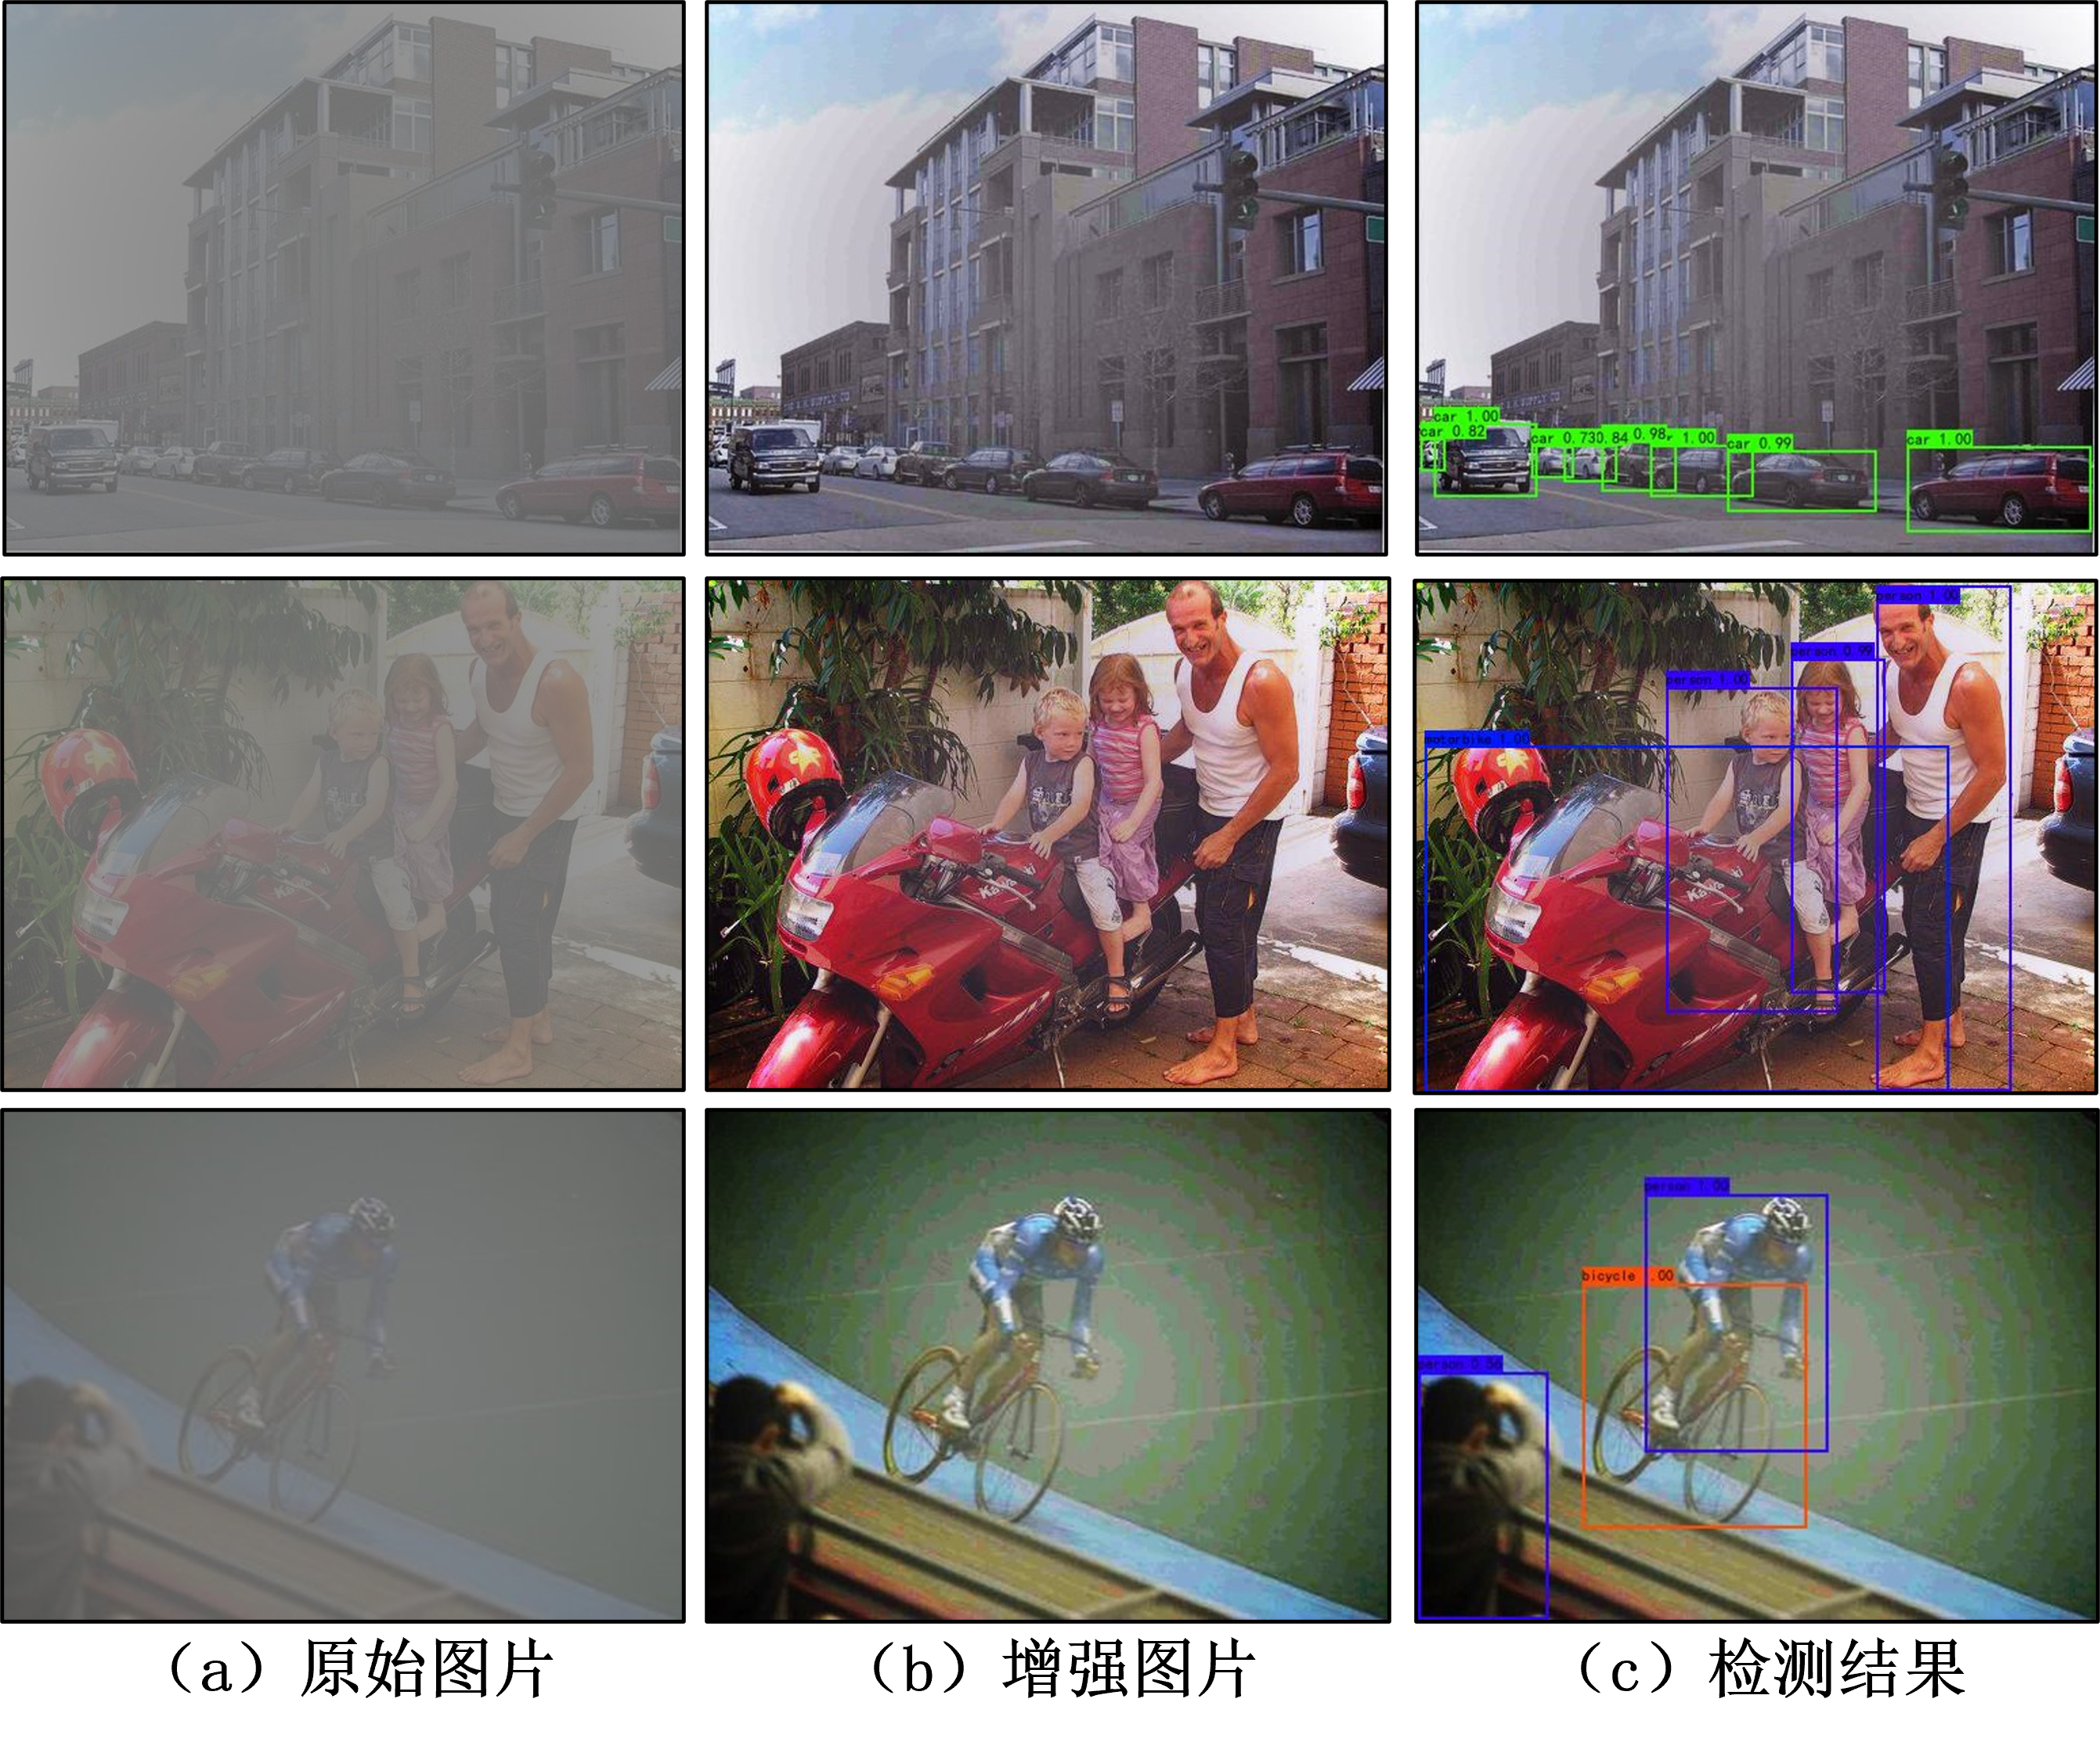
\includegraphics[width=13cm]{chapter4/18.png}
    \caption{\label{fig:ch4_18}DPFE-YOLO在VOC\_fog测试集上的部分增强与检测结果}
\end{figure}

\begin{figure}[htbp]
    \centering
    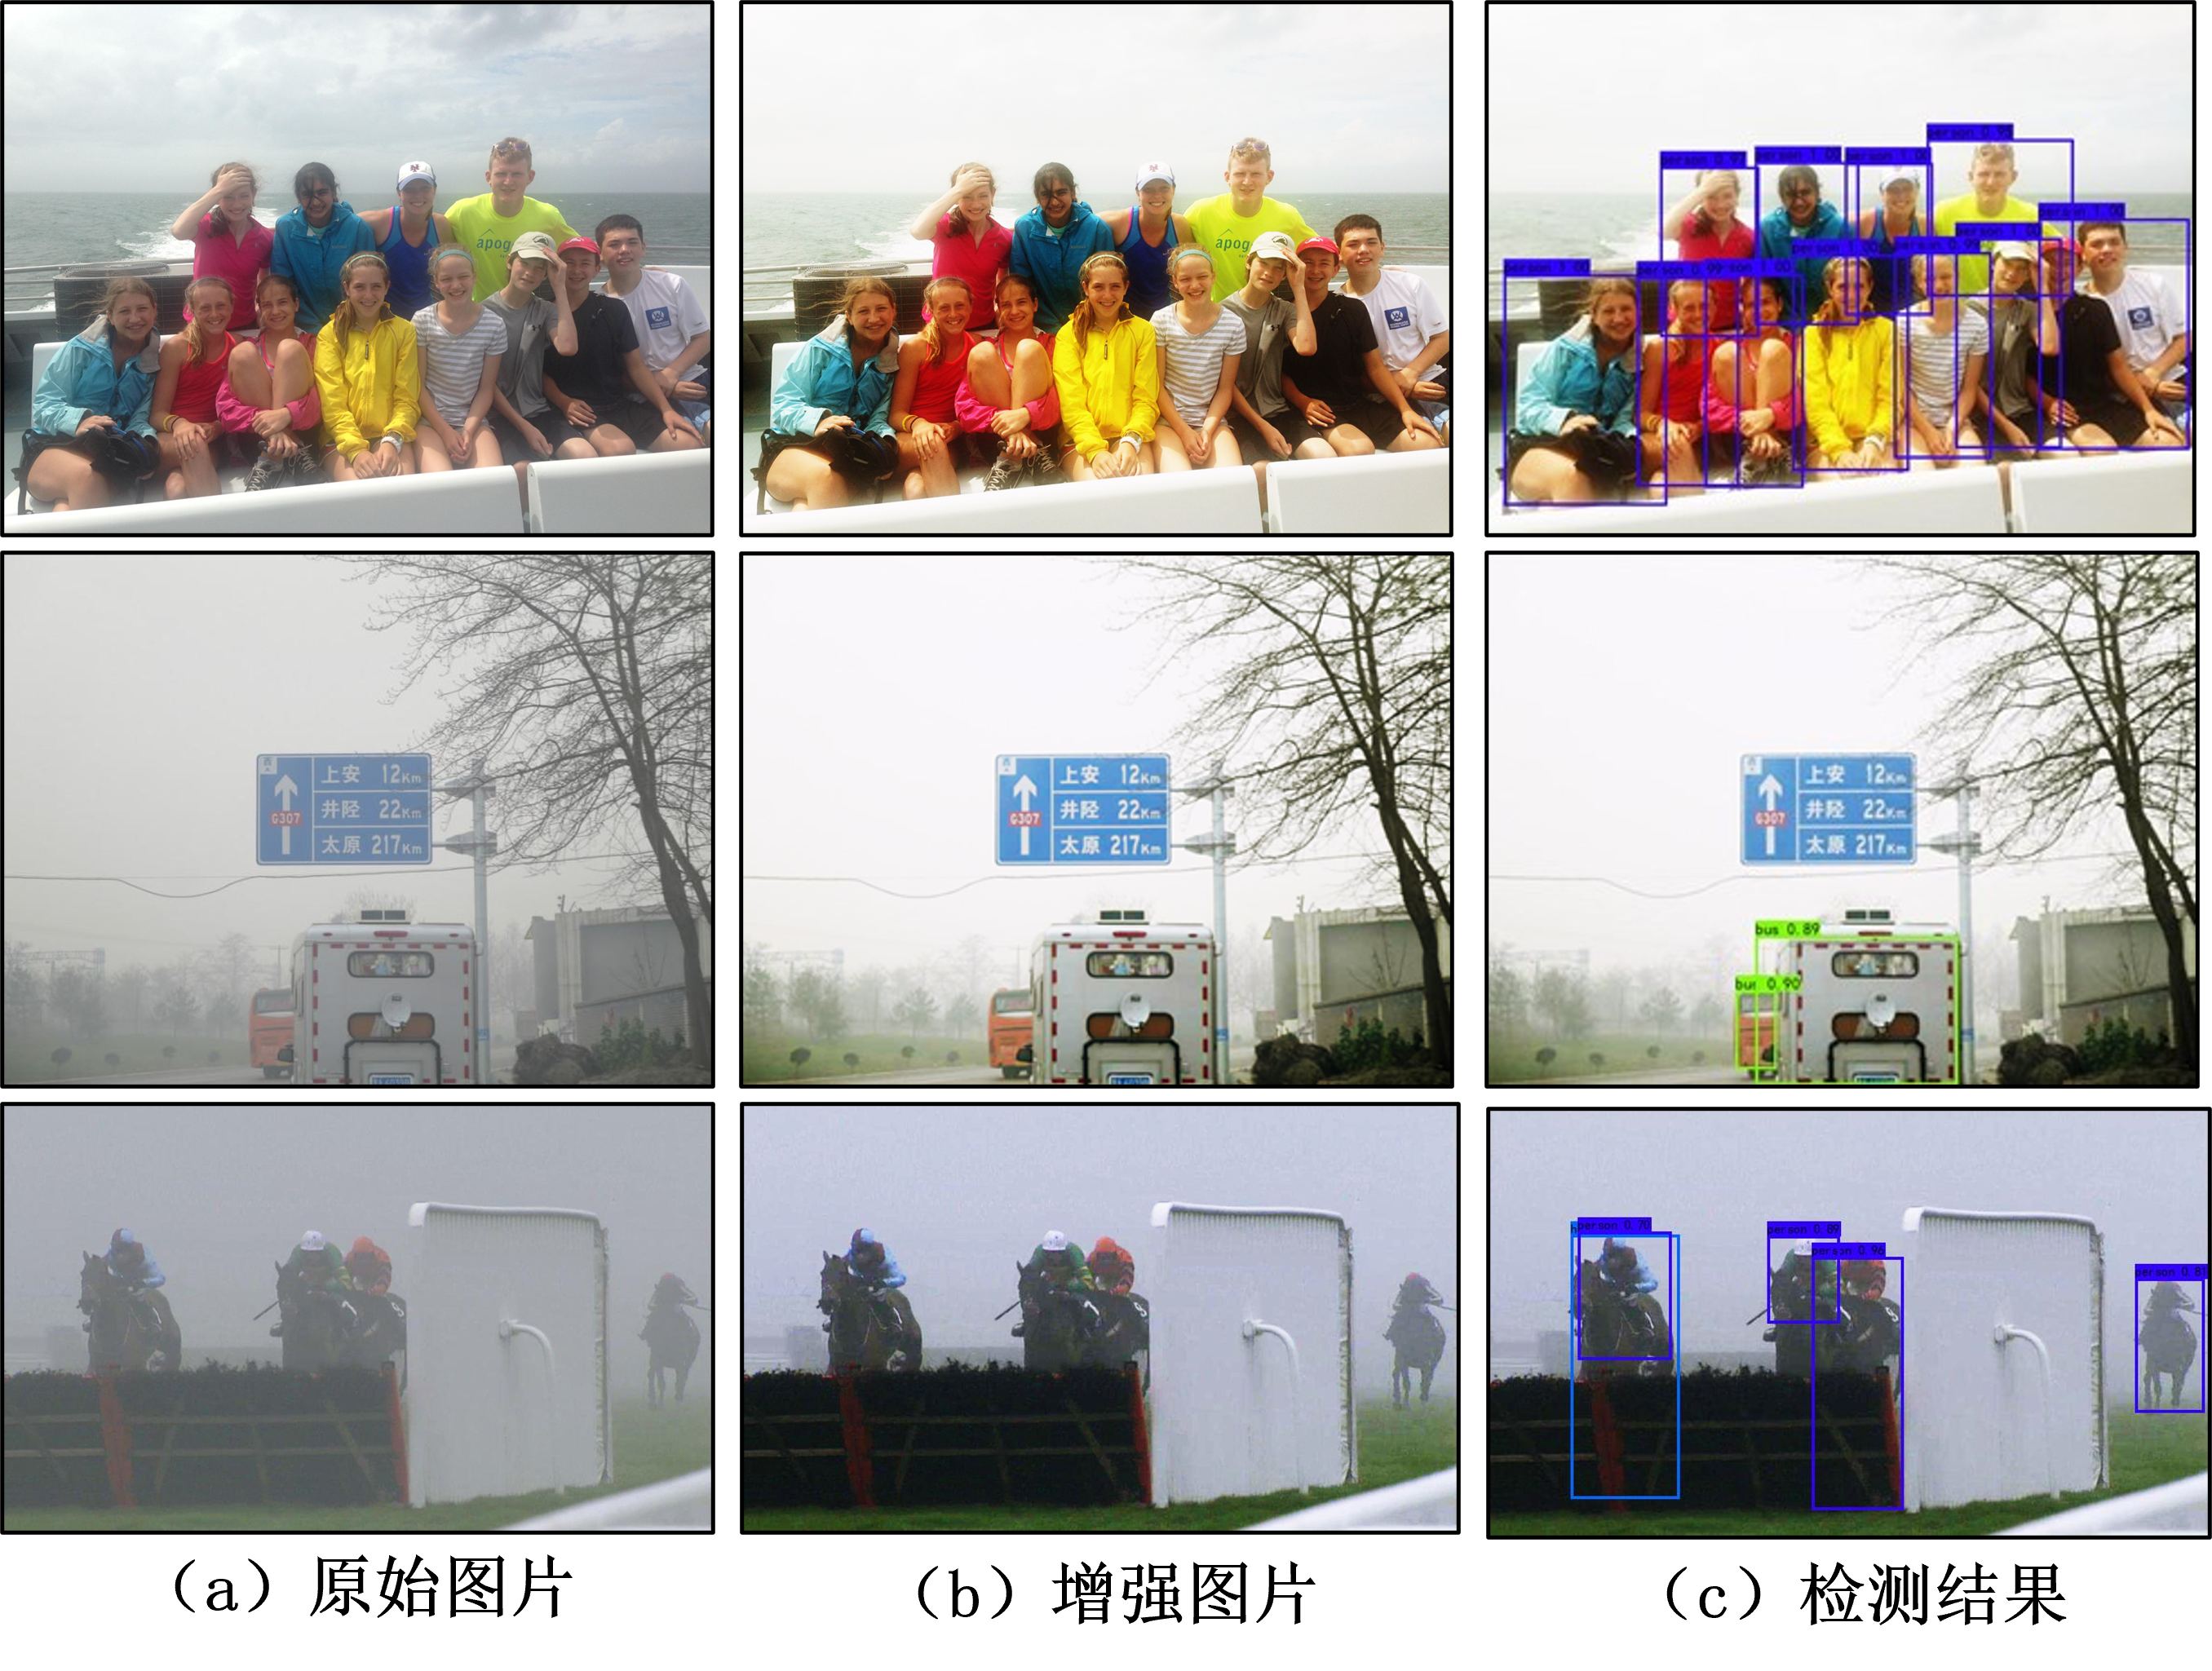
\includegraphics[width=13cm]{chapter4/19.png}
    \caption{\label{fig:ch4_19}DPFE-YOLO在RTTS测试集上的部分增强与检测结果}
\end{figure}

\subsection{自适应增强模块消融实验}
\label{subsec:ch4_4_3}
为了深入验证 DPFE-YOLO 框架中关键组件的有效性以及超参数设定的合理性,本节在弱光跨域场景(VOC\_dark 与 ExDark)下开展了一系列消融实验。
实验主要围绕以下三个核心方面展开:双流滤波块(DFB)的级联深度、视觉编码器(Vision Encoder)的结构设计以及门控融合策略。

\textbf{1. DFB级联深度的影响}

DPFE 采用渐进式架构,通过级联$N$个 DFB 逐步恢复图像质量。级联深度$N$直接决定了模型的非线性映射能力与特征恢复的精细度。
表\ref{tab:dfb_num_ablation}展示了当级联层数$N$从1增加至6时,模型在合成域与真实域上的检测性能变化。
\begin{table}[htbp]
    \centering
    \caption{双流滤波块(DFB)级联数量 $N$ 对检测性能的消融实验}
    \label{tab:dfb_num_ablation}
    \resizebox{0.6\linewidth}{!}{
        \begin{tabular}{ccc}
            \toprule
            \textbf{级联层数 ($N$)} & \textbf{VOC\_dark (Syn)  $\uparrow$} & \textbf{ExDark (Real)  $\uparrow$} \\ \midrule
            1                   & 80.88                   & 56.67                 \\
            2                   & 81.07                   & 56.48                 \\
            3                   & 81.17                   & 57.15                 \\
            4                   & 80.90                   & 57.22                 \\
            \textbf{5 (Default)} & \textbf{81.29}          & 57.32                 \\
            6                   & 81.08                   & \textbf{57.41}        \\ \bottomrule
        \end{tabular}
        }
\end{table}
    
定量结果显示,当 $N=5$ 时,模型在合成与真实弱光数据集上取得了最优或接近最优的综合性能。
为了更深入地理解不同深度对增强效果的影响,我们计算了各增强结果与真值图像(GroundTruth,GT)的差分热力图,如\autoref{fig:ch4_20}所示。
热力图中,蓝色区域表示增强图像与GT差异较小,绿色/黄色区域表示存在差异。

从热力图的变化中可以观察到渐进式增强的演进过程:
当$N=1$时,热力图显示小狗身体区域绿色较多,人物身上也有浅绿色,表明单级增强的结果与GT仍存在较大差异。
随着$N$增加至2和3,热力图显示小狗身体区域大面积转为蓝色,仅在鼻子、眼睛等细节处保留绿色;
人物区域也以浅绿色为主,表明增强效果逐步逼近GT。
当$N$增加至4和5时,人物区域的绿色进一步减少,蓝色区域增加,整体与GT的差异持续缩小。
特别地,当$N=5$时,热力图显示除边缘少量绿色外,大部分区域呈现蓝色,表明增强图像在整体和细节上均与GT最为接近。
然而,当$N=6$时,热力图与$N=4$时相似,未显示出进一步的改善,这与定量指标中性能的轻微波动相符。
\begin{figure}[htbp]
\centering
\includegraphics[width=15cm]{chapter4/20.png}
\caption{\label{fig:ch4_20}不同级联层数($N=1,2,3,4,5,6$)下增强图像与真值图像的差分热力图对比}
\end{figure}

这一现象验证了渐进式增强架构的设计动机:适度的级联深度($N=5$)允许网络分阶段、由粗到细地恢复图像,
而深度不足则恢复不充分,过度增加深度可能导致性能增益减小并引入冗余计算。因此,我们最终选择$N=5$作为标准配置,在性能与效率间取得最佳平衡。

\textbf{2. 视觉编码器结构的影响}

为验证所提出的全卷积视觉编码器的有效性,
我们将其与一个精心设计的基线编码器进行对比。
该基线编码器参考了ERUP-YOLO的核心思想并扩展为多尺度结构:
它使用平均池化进行下采样,并在每个特征尺度后接入独立的全连接层,
为每一级DFB预测增强参数。
此设计旨在与我们的方法进行对等比较。消融实验结果如\autoref{tab:encoder_ablation}所示。
\begin{table}[htbp]
\centering
\caption{视觉编码器结构对检测性能的消融实验}
\label{tab:encoder_ablation}
\resizebox{0.8\linewidth}{!}{
\begin{tabular}{ccc}
\toprule 
\textbf{视觉编码器} & \textbf{VOC\_dark (Syn)  $\uparrow$} & \textbf{ExDark (Real)  $\uparrow$} \\ \midrule
多尺度+全连接层(基线)        & 70.74                   & 50.41                 \\
\textbf{全卷积编码器(Ours)}    & \textbf{81.29}          & \textbf{57.32}        \\ \bottomrule
\end{tabular}
}
\end{table}

实验结果表明,即使基线编码器采用了多尺度设计,其性能仍显著低于我们的全卷积编码器,在VOC\_dark和ExDark上的mAP分别落后10.55和6.91个百分点。
这一显著差距反映出,即便在多尺度条件建模的框架下,编码器的具体实现方式对退化感知的准确性与增强参数预测的质量产生着决定性影响。
相比之下,我们设计的全卷积视觉编码器有效缓和固定池化带来的高频信息丢失问题,
并通过卷积下采样与逐层特征映射,
为每一层 DFB 提供更加稳定且具判别性的条件向量,
从而在弱光场景下获得了更优的增强质量与检测性能。

\textbf{3. 门控融合机制的影响}

DPFE中门控网络的作用是自适应地融合贝塞尔像素级滤波(BPW)与基于核的局部滤波(KBL)两条路径的输出。
为验证其自适应性优势,我们将其与多种固定的权重分配策略进行比较,结果如表\ref{tab:gate_ablation}所示。
\begin{table}[htbp]
\centering
\caption{门控融合策略对检测性能的消融实验}
\label{tab:gate_ablation}
\resizebox{0.7\linewidth}{!}{
\begin{tabular}{cccc}
\toprule
\textbf{权重比例 (BPW : KBL)} & \textbf{VOC\_dark (Syn) $\uparrow$} & \textbf{ExDark (Real) $\uparrow$} \\ \midrule
0 : 10 (Only KBL)            & 65.06                   & 49.47                 \\
2 : 8                        & 67.90                   & 55.00                 \\
4 : 6                        & 66.61                   & 54.17                 \\
5 : 5 (Average)              & 69.69                   & 55.63                 \\
6 : 4                        & 70.77                   & 55.26                 \\
8 : 2                        & 71.64                   & 56.04                 \\
10 : 0 (Only BPW)            & 72.16                   & 56.04                 \\ 
\textbf{Adaptive Gate (Ours)} & \textbf{81.29}          & \textbf{57.32}        \\ \bottomrule
\end{tabular}
}
\end{table}

通过详细分析表\ref{tab:gate_ablation},可以得出以下关键结论:
\begin{itemize}
    \item \textbf{单一机制的局限性}:仅使用局部核滤波(0:10)的效果最差,说明在严重弱光下,首要任务是恢复可见度;仅使用贝塞尔增强(10:0)效果尚可,但仍低于最终方案,说明缺乏去噪和边缘锐化会导致检测精度受限。
    \item \textbf{固定比例的次优性}:在固定比例的实验中,偏向光照恢复的配置(如 8:2, 10:0)普遍优于偏向滤波的配置。然而,即便是表现最好的固定比例(10:0 或 8:2),其 mAP 仍显著低于自适应门控机制(VOC 上差距超过 9\%)。
    \item \textbf{自适应融合的优越性}:自适应的门控机制能够根据输入特征的语义内容,动态决定每个像素点更需要“提亮”还是“去噪”。这种像素级的动态权衡是任何固定硬编码策略无法比拟的,从而使得 DPFE 能够在复杂多变的弱光环境中始终保持最优的增强效果。
\end{itemize}

\subsection{跨域多目标跟踪鲁棒性评估}
\label{subsec:ch4_4_4}
为验证\ref{sec:ch4_3}节中所构建的完整跨域跟踪系统的鲁棒性,我们在合成跨域数据上进行了控制变量实验。
实验设置如\ref{subsec:ch4_4_1}节所述:以MOT17清晰视频为源域基准,并构建其弱光(MOT17\_dark)与雾天(MOT17\_fog)退化版本。
后端跟踪器固定为在清晰域上预训练的DGCTracker。前端采用统一的检测器(来自弱光训练DPFE-YOLO的YOLOv3权重),以隔离增强模块的影响。

具体的实验流程如下:

\textbf{1. 基准测试}:在清晰的MOT17视频序列上,使用YOLOv3检测器与DGCTracker组合进行测试,获得系统在理想条件下的性能基准。

\textbf{2. 弱光与雾天退化测试}:在合成的退化数据集MOT17\_dark与MOT17\_fog上,使用完全相同的检测-跟踪系统进行测试,以评估视觉退化对整体跟踪链路的冲击。

\textbf{3. 增强恢复测试}:分别在MOT17\_dark与MOT17\_fog数据上,在检测器前端集成对应的DPFE增强模块(即完整DPFE-YOLOv3),再次进行跟踪测试,以验证所提增强方案对跨域跟踪性能的恢复能力。

如表\ref{tab:mot_cross_domain}所示,
当测试环境从清晰域变为恶劣域时,所有跟踪指标均显著下降。
在弱光环境下(MOT17\_dark),HOTA与MOTA分别较清晰域下降5.62与5.61个百分点;
在雾天环境下(MOT17\_fog),性能退化更为严重,HOTA与MOTA分别下降11.62与12.20个百分点。
这一结果证实了视觉退化会严重损害检测质量(DetA下降),进而破坏轨迹关联(AssA、IDF1下降),最终导致整体跟踪性能的崩溃。

在引入对应的DPFE前端增强模块后,跟踪性能得到了有效恢复。
在弱光场景中,增强后(MOT17\_dedark)的HOTA回升至38.08,MOTA恢复至31.04,均接近清晰域基准水平。
在雾天场景中,增强后(MOT17\_defog)的HOTA与MOTA较未增强时分别提升了7.11与7.45个百分点。
值得注意的是,增强后身份保持相关指标(IDF1、IDR、IDP)均得到明显改善,表明更清晰稳定的外观特征有效缓解了身份混淆问题。
\begin{table}[htbp]
\centering
\caption{跨域条件下多目标跟踪系统鲁棒性评估}
\label{tab:mot_cross_domain}
\resizebox{0.95\linewidth}{!}{
\begin{tabular}{ccccccccc}
\toprule
\textbf{Test Domain} & \textbf{HOTA} $\uparrow$ & \textbf{DetA} $\uparrow$ & \textbf{AssA} $\uparrow$ & \textbf{IDF1} $\uparrow$ & \textbf{IDR} $\uparrow$ & \textbf{IDP} $\uparrow$ & \textbf{MOTA} $\uparrow$ & \textbf{MOTP} $\uparrow$ \\ \midrule
\textbf{MOT17 (Clear)} & 38.87 & 27.01 & 57.11 & 44.34 & 30.66 & 80.07 & 31.23 & 76.21 \\ \midrule
MOT17\_dark            & 33.25 & 22.30 & 50.48 & 35.66 & 23.36 & 75.31 & 25.62 & \textbf{76.61} \\
\textbf{MOT17\_dedark} & \textbf{38.08} & \textbf{26.42} & \textbf{56.18} & \textbf{43.05} & \textbf{29.53} & \textbf{79.42} & \textbf{31.04} & 76.11 \\ \midrule
MOT17\_fog             & 27.25 & 17.56 & 43.11 & 28.11 & 17.62 & 69.54 & 19.03 & 75.56 \\
\textbf{MOT17\_defog}  & \textbf{34.36} & \textbf{23.39} & \textbf{51.37} & \textbf{37.79} & \textbf{25.17} & \textbf{75.87} & \textbf{26.48} & 75.72 \\ \bottomrule
\end{tabular}
}
\end{table}

为直观展示增强模块对跟踪稳定性的贡献,图\ref{fig:ch4_21}展示了MOT17-05序列在弱光场景下的跟踪结果对比。
在未增强的弱光图像(图\ref{fig:ch4_21}(a))中,
目标(如ID \#3)因严重的光照不足导致其外观特征退化、判别性显著降低。
这使得基于表观特征的嵌入表示与关联过程变得不稳定,进而引发明显的身份跳变现象——ID \#3在相邻帧中被错误地分配给了不同行人。
而在经过DPFE增强后(图\ref{fig:ch4_21}(b)),图像的整体亮度与局部对比度得到有效改善,
人物目标的轮廓与纹理细节更为清晰。
由此获得的特征表示判别力更强、一致性更高,
使得跟踪器能够稳定地保持ID \#3的身份连续性,未出现跳变。
这一对比结果证明,DPFE模块通过有效改善输入图像质量、恢复具有高判别性的视觉特征,显著增强了跟踪系统在跨域恶劣环境下的身份保持鲁棒性。
\begin{figure}[htbp]
\centering
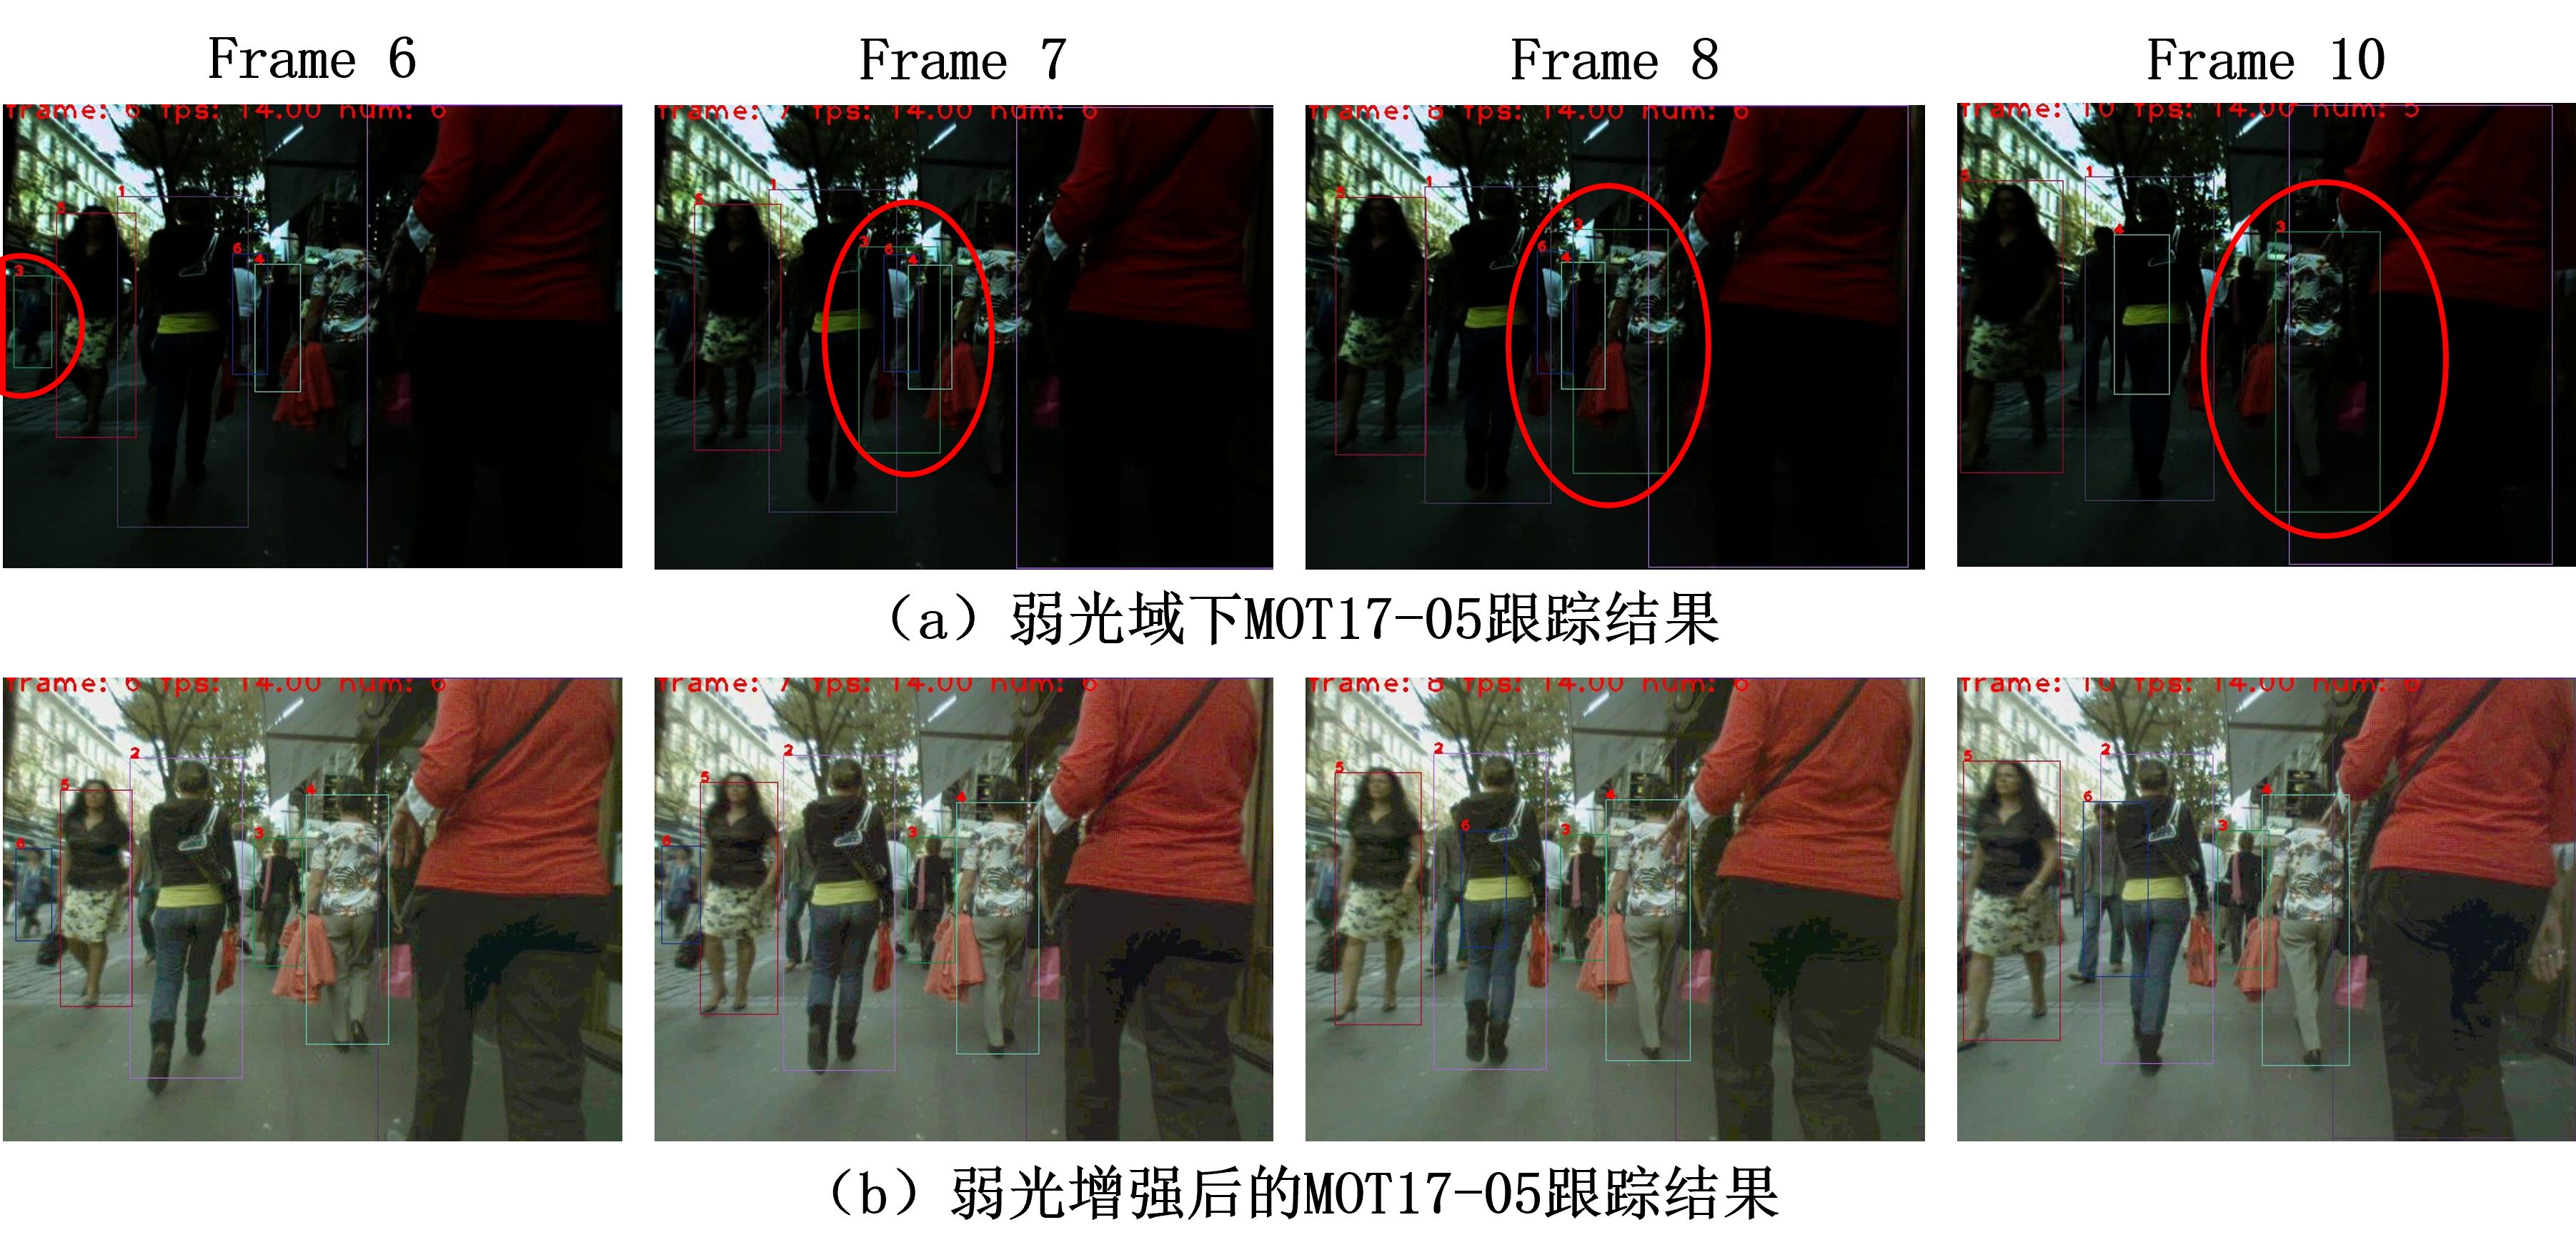
\includegraphics[width=15cm]{chapter4/21.png}
\caption{\label{fig:ch4_21}跨域跟踪结果可视化对比(MOT17-05)}
\end{figure}

\subsection{系统效率与工程优势分析}
\label{subsec:ch4_4_5}
衡量一个多目标跟踪系统在实际工程部署中的潜力,除了跟踪精度外,其计算效率、资源占用以及架构的灵活性同样是关键的评价标准。
为验证本章所构建的跨域自适应跟踪系统的工程可用性,我们在 NVIDIA RTX 3090 平台上对系统各模块进行了定量测试。

系统测试涵盖了前端增强器(DPFE)、检测器(YOLOv3)以及跟踪器(DGCTracker),各模块的参数量与推理速度如\autoref{tab:system_efficiency}所示。
\begin{table}[htbp]
\centering
\caption{系统各模块参数量与推理速度性能分析(测试环境:NVIDIA RTX 3090)}
\label{tab:system_efficiency}
\resizebox{0.9\linewidth}{!}{
\begin{tabular}{cccc}
\toprule
\textbf{指标 / 模块} & \textbf{增强器 (DPFE)} & \textbf{检测器 (YOLOv3)} & \textbf{跟踪器 (DGCTracker)} \\ 
\midrule
\textbf{参数量 (Params)} & \textbf{9.85 M} & 61.63 M & 27.28 M \\  
\midrule
\textbf{480P 推理速度} & \textbf{263 FPS} & 64 FPS & 68 FPS \\
\textbf{1080P 推理速度} & \textbf{217 FPS} & 55 FPS & 30 FPS \\
\bottomrule
\end{tabular}
}
\end{table}

基于上述定量数据,本章提出的框架在工程落地方面展现出以下三大核心优势:

\textbf{1. 极低的额外参数开销(轻量化优势)}

从存储与显存占用的角度看,引入的自适应增强模块(DPFE)体现了显著的轻量化设计。
其参数量仅为9.85 M,约为检测器(YOLOv3)参数量的16\%,仅占整个系统总参数量的不到 10\%。
这一数据表明,在现有的检测跟踪流水线中引入该前端增强功能,几乎不会带来显著的存储与加载压力。
这种以极小的参数代价换取强大的跨域环境适应能力的设计,使其非常适合部署在对存储空间敏感的嵌入式设备或边缘计算终端中。

\textbf{2. 卓越的实时处理效率(速度优势)}

在推理速度方面,DPFE模块展现了极高的处理效率。
在480P与1080P分辨率下,其单帧处理速度分别达到263 FPS与217 FPS,远高于后端检测器与跟踪器。
在串行处理流程中,前端增强模块不会成为系统的计算瓶颈。
即使后端跟踪器在1080P下以约30 FPS运行,系统整体仍能满足实时视频流(通常为25-30 FPS)的处理需求。

\textbf{3. 灵活的模块化扩展架构(工程优势)}

得益于“增强-检测-跟踪”的模块化解耦设计,该系统具备良好的可扩展性与兼容性。
前端DPFE模块输出标准RGB图像,因此其后端的检测模块可以灵活替换为任何先进的检测器(如YOLOv8\cite{v8}、RT-DETR\cite{rt—detr}等),而无需重新设计或训练增强网络。
这种设计赋予了系统持续演进的能力,并能针对不同的硬件平台或精度要求进行快速适配,显著降低了系统升级与维护的成本。

综上所述,本章构建的跨域自适应多目标检测与跟踪系统不仅在算法层面实现了对恶劣视觉条件的鲁棒感知,
在工程层面也展现出高实时性、低资源消耗与强可扩展性的综合优势,
为其在智能交通、视频监控等对可靠性与实时性要求严苛的实际场景中的部署应用奠定了坚实基础。
\section{本章小结}
\label{sec:ch4_5}
本章聚焦于多目标跟踪系统在真实开放场景下面临的跨域自适应问题,重点研究了恶劣天气(如雾天、弱光等)条件下检测与跟踪性能退化机理,
并提出了一套完整的前端自适应增强解决方案,旨在从输入层面缓解域偏移,提升系统在跨域环境中的鲁棒性。

本章首先从数据分布、检测响应与跟踪关联三个层面系统分析了恶劣环境对多目标跟踪系统的退化机制,
明确了前端检测质量对整体跟踪性能的决定性影响。
在此基础上,提出了基于双渐进滤波增强器(DPFE)的跨域自适应增强检测框架(DPFE-YOLO),
通过可学习的全局像素映射与局部结构滤波,结合门控融合与渐进式级联机制,实现对退化图像的自适应恢复。

在方法设计上,本章详细阐述了DPFE的视觉编码器与双流滤波块结构,
提出了增强-检测端到端协同训练策略,并引入多任务损失函数确保增强过程在提升检测性能的同时保持视觉自然性。
进一步地,将训练好的增强-检测模块与第三章提出的跟踪器(DGCTracker)集成,构建了完整的“增强-检测-跟踪”跨域自适应推理框架。

通过系统的实验验证,本章所提方法在跨域目标检测任务上显著超越了现有先进方法,
在合成与真实退化数据集上均表现出优越的检测精度与视觉增强效果。
消融实验证实了渐进式架构、全卷积编码器及自适应门控机制的有效性。
在跨域多目标跟踪评估中,集成DPFE前端增强的系统在恶劣环境下有效缓解了轨迹碎片化与身份混淆问题,显著恢复了跟踪性能。
此外,系统在参数量、推理速度与模块化扩展性方面表现出良好的工程优势,具备在实际场景中部署的潜力。
